\section{\texorpdfstring{$G$}{G}-invariance and \texorpdfstring{$G$}{G}-admissiblity of finite type}
\label{section:invariance and admissibility}

In this section, we will provide a proof of Theorem~\ref{theorem:G-invariance and G-admissibility}. 
\begin{lemma}\label{lemma:no weird cycles in An}
Let $\quiver$ be a quiver of type $\dynA_{2n-1}$.
Suppose that $\quiver$ is invariant under an action of $G = \Z/2\Z$ defined by 
\begin{align*}
\tau(i)&=2n-i
\end{align*}
for all $i\in[2n-1]$. Here, we denote by $\tau \in \Z/2\Z$ the generator of $G$.
Then there is no oriented cycle of the form
\[
j\to i\to\tau(j)\to\tau(i)\to j
\]
for any $i,j\neq n$.
\end{lemma}
\begin{proof}
It is well known that a quiver $\quiver$ of type $\dynA$ corresponds to a triangulation of a polygon, where diagonals and triangles define mutable vertices and arrows.
Therefore, any minimal cycle in $\quiver$ if exists is of length $3$, which is also proved in~\cite[\S2]{BuanVatne08}.
Hence if an oriented cycle $j\to i\to\tau(j)\to\tau(i)\to j$ of length $4$ exists, then there must be an edge $i-\tau(i)$ or $j-\tau(j)$ in $\quiver$. Hence $b_{i,\tau(i)}\neq0$ or $b_{j,\tau(j)}\neq0$ for $\qbasispr=(b_{k,\ell})=\qbasispr(\quiver)$.

This is impossible because $\quiver$ is $\Z/2\Z$-invariant and so
\[
b_{i,\tau(i)} = b_{\tau(i),\tau(\tau(i))} = b_{\tau(i), i} = -b_{i,\tau(i)}\quad\Longrightarrow\quad
b_{i,\tau(i)}=0.
\]
Therefore we are done.
\end{proof}


\begin{proposition}\label{proposition:admissibility for An}
Let $\quiver$ be a quiver of type $\dynA_{2n-1}$, which is $\Z/2\Z$-invariant as above. Then $\quiver$ is $\Z/2\Z$-admissible.
\end{proposition}
\begin{proof}
We will check the conditions~\eqref{mutable},~\eqref{bii'=0}, and~\eqref{nonnegativity_of_bijbi'j} for the admissibility according to Definition~\ref{definition:admissible quiver}.
Let $\qbasispr = (b_{i,j}) = \qbasispr(\quiver)$. 

\noindent \eqref{mutable} Since all vertices in $\quiver$ are mutable, the condition~\eqref{mutable} is obviously satisfied.

\noindent \eqref{bii'=0} On the other hand, for each $i\in[2n-i]$, we have 
\[
b_{i,\tau(i)}=(\cycle_i, \cycle_{\tau(i)})= (\cycle_{\tau(i)}, \cycle_{\tau(\tau(i))}) = (\cycle_{\tau(i)}, \cycle_i) = -b_{i,\tau(i)},
\]
which implies  
\[
b_{i,\tau(i)}=0.
\]

\noindent \eqref{nonnegativity_of_bijbi'j} Finally, we need to prove that for each $i, j$,
\[
b_{i,j}b_{\tau(i),j}\ge 0.
\]

If $j=n$, then since $\tau(n)=n$, we have
\[
b_{i,n}b_{\tau(i),n}=b_{i,n}b_{\tau(i),\tau(n)} = b_{i,n}b_{i,n}\ge 0.
\]
Similarly, if $i=n$, then 
\[
b_{n, j}b_{\tau(n),j} = b_{n,j}b_{n,j}\ge 0.
\]

Suppose that for some $i, j\neq n$,
\[
b_{i,j}b_{\tau(i),j}<0.
\]
By changing the roles of $i$ and $\tau(i)$ if necessary, we may assume that $b_{i,j}<0<b_{\tau(i),j}$.
Then we also have
\[
b_{\tau(i),\tau(j)}<0<b_{i,\tau(j)},
\]
which implies that there is an oriented cycle in $\quiver$
\[
j\to i \to \tau(j) \to \tau(i) \to j.
\]
However, this contradicts to Lemma~\ref{lemma:no weird cycles in An} and therefore $\quiver$ satisfies all conditions in Definition~\ref{definition:admissible quiver}.
\end{proof}


\begin{proposition}\label{proposition:admissibility for D4}
Let $\quiver$ be a quiver on $[4]$ of type $\dynD_{4}$, which is invariant under the $\Z/3\Z$-action given by
\begin{align*}
1&\stackrel{\tau}{\longleftrightarrow} 1,& 2&\stackrel{\tau}{\longrightarrow} 3\stackrel{\tau}{\longrightarrow} 4\stackrel{\tau}{\longrightarrow} 2.
\end{align*}
Here, we denote by $\tau$ the generator of $\Z/3\Z$.
Then the quiver $\quiver$ is $\Z/3\Z$-admissible.
\end{proposition}
\begin{proof}
\noindent \eqref{mutable} This is obvious as before.

\noindent \eqref{bii'=0} Let $\qbasispr=(b_{i,j})=\qbasispr(\quiver)$. Suppose that $b_{2,3}\neq0$. Since the quiver is $\Z/3\Z$-invariant,
\[
b_{2,3}=b_{3,4}=b_{4,2}\neq0
\]
and so $\quiver$ has a directed cycle either
\[
2\to3\to4\to 2\quad\text{or}\quad 2\to4\to3\to 2.
\]
Then according to the value $b_{1,2}$, the underlying graph of the quiver $\quiver$ is either the complete graph $K_4$ or a disconnected graph.
However, both are impossible as shown in~\cite[Figure~1]{BuanTorkildsen09}. 
Therefore, we obtain
\[
b_{2,3}=b_{3,4}=b_{4,2}=0.
\]

\noindent \eqref{nonnegativity_of_bijbi'j} The only entries we need to check are $b_{1,j}$'s, which are all equal by the $\Z/3\Z$-invariance of $\quiver$. Therefore
\[
b_{1,j}b_{1,j'}\ge 0.
\]
This completes the proof.
\end{proof}


\begin{lemma}\label{lemma:no weird cycles in E6}
Let $\quiver$ be a quiver on $[6]$ of type $\dynE_6$, which is invariant under the $\Z/2\Z$-action defined by
\begin{align*}
i&\stackrel{\eta}{\longleftrightarrow} i, i\le 2,&
3&\stackrel{\eta}{\longleftrightarrow} 5,&
4&\stackrel{\eta}{\longleftrightarrow} 6.
\end{align*}
Here, we denote by $\eta$ the generator of $\Z/2\Z$.
Then there is no oriented cycle, which is either
\begin{equation}\label{eq_weird_cycles_in_E6}
3\to4\to5\to6\to3\quad\text{or}\quad
3\to6\to5\to4\to3.
\end{equation}
\end{lemma}
\begin{proof}
We first recall from~\cite[Theorem~1.8]{FZ2_2003} that 
\begin{equation}\label{equation_bij_le_1}
|b_{i,j}|\le 1 \qquad \text{ for all }i,j\in[6].
\end{equation} 
Otherwise, $\quiver$ produces a cluster pattern of infinite type.
Hence, $\quiver$ is a simple directed graph.

Suppose that $\quiver$ contains an oriented cycle in~\eqref{eq_weird_cycles_in_E6}.
By relabeling if necessary, we may assume that the $\quiver$ contains an oriented cycle $3\to4\to5\to6\to 3$.
Then, since $\quiver$ is connected, at least one of vertices $1$ and $2$ is joined with one of vertices $3,4,5$ and $6$ by an edge.
Without loss of generality, we may assume that such a vertex is $1$.

Let $\quiver'$ be the quiver on $\{1,3,4,5,6\}$ obtained by forgetting the vertex $2$ in $\quiver$.
Then, by the invariance of $\quiver$ under $\Z/2\Z$-action, 
\begin{align*}\label{equation:squares}
\quiver' = 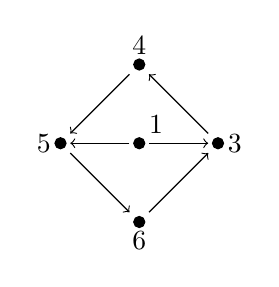
\begin{tikzpicture}[baseline=-.5ex]
\begin{scope}
\draw[fill] (0,0) node (A1) {} circle (2pt)
(0,1) node (A4) {} circle (2pt)
(-1,0) node (A5) {} circle (2pt) 
(0,-1) node (A6) {} circle (2pt) 
(1,0) node (A7) {} circle (2pt);
\draw[->] (A1) node[above right] {$1$} -- (A5);
\draw[->] (A1) -- (A7);
\draw[->] (A4) -- (A5) node[left] {$5$};
\draw[->] (A5) -- (A6) node[below] {$6$};
\draw[->] (A6) -- (A7) node[right] {$3$};
\draw[->] (A7) -- (A4) node[above] {$4$};
\end{scope}
\end{tikzpicture}, \quad
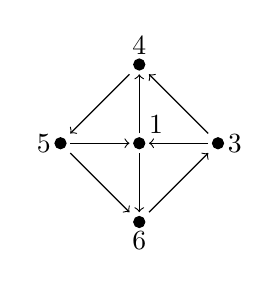
\begin{tikzpicture}[baseline=-.5ex]
\begin{scope}[xshift=3cm]
\draw[fill] (0,0) node (A1) {} circle (2pt)
(0,1) node (A4) {} circle (2pt)
(-1,0) node (A5) {} circle (2pt) 
(0,-1) node (A6) {} circle (2pt) 
(1,0) node (A7) {} circle (2pt);
\draw[->] (A1) node[above right] {$1$} -- (A4);
\draw[->] (A1) -- (A6);
\draw[->] (A5) -- (A1);
\draw[->] (A7) -- (A1);
\draw[->] (A4) -- (A5) node[left] {$5$};
\draw[->] (A5) -- (A6) node[below] {$6$};
\draw[->] (A6) -- (A7) node[right] {$3$};
\draw[->] (A7) -- (A4) node[above] {$4$};
\end{scope}
\end{tikzpicture},\quad\text{ or }\quad
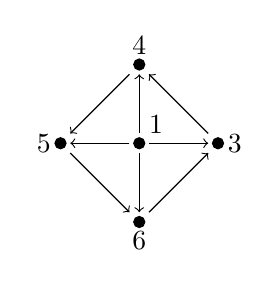
\begin{tikzpicture}[baseline=-.5ex]
\begin{scope}[xshift=6cm]
\draw[fill] (0,0) node (A1) {} circle (2pt)
(0,1) node (A4) {} circle (2pt)
(-1,0) node (A5) {} circle (2pt) 
(0,-1) node (A6) {} circle (2pt) 
(1,0) node (A7) {} circle (2pt);
\draw[->] (A1) node[above right] {$1$} -- (A4);
\draw[->] (A1) -- (A5);
\draw[->] (A1) -- (A6);
\draw[->] (A1) -- (A7);
\draw[->] (A4) -- (A5) node[left] {$5$};
\draw[->] (A5) -- (A6) node[below] {$6$};
\draw[->] (A6) -- (A7) node[right] {$3$};
\draw[->] (A7) -- (A4) node[above] {$4$};
\end{scope}
\end{tikzpicture}
\subset \quiver
\end{align*}
up to relabeling and the mutation $\mutation_1$.
Then, via further mutations, each of these quivers can be transformed to a quiver producing a cluster pattern of infinite type because of the condition~\eqref{equation_bij_le_1} as follows:
\begin{align*}
&\begin{tikzpicture}[baseline=-.5ex]
\begin{scope}
\draw[fill] (0,0) node (A1) {} circle (2pt)
(0,1) node (A4) {} circle (2pt)
(-1,0) node (A5) {} circle (2pt) 
(0,-1) node (A6) {} circle (2pt) 
(1,0) node (A7) {} circle (2pt);
\draw[->] (A1) node[above right] {$1$} -- (A5);
\draw[->] (A1) -- (A7);
\draw[->] (A4) -- (A5) node[left] {$5$};
\draw[->] (A5) -- (A6) node[below] {$6$};
\draw[->] (A6) -- (A7) node[right] {$3$};
\draw[->] (A7) -- (A4) node[above] {$4$};
\end{scope}
\begin{scope}[xshift=5cm]
\draw[fill] (0,0) node (A1) {} circle (2pt)
(0,1) node (A4) {} circle (2pt)
(-1,0) node (A5) {} circle (2pt) 
(0,-1) node (A6) {} circle (2pt) 
(1,0) node (A7) {} circle (2pt);
\draw[->] (A1) node[above right] {$1$} -- (A4);
\draw[->] (A1) -- (A6);
\draw[->] (A5) -- (A1);
\draw[->] (A7) -- (A1);
\draw[->] (A4) -- (A5) node[left] {$5$};
\draw[->] (A5) -- (A6) node[below] {$6$};
\draw[->] (A6) -- (A7) node[right] {$3$};
\draw[->] (A7) -- (A4) node[above] {$4$};
\end{scope}
\begin{scope}[xshift=10cm]
\draw[fill] (0,0) node (A1) {} circle (2pt)
(0,1) node (A4) {} circle (2pt)
(-1,0) node (A5) {} circle (2pt) 
(0,-1) node (A6) {} circle (2pt) 
(1,0) node (A7) {} circle (2pt);
\draw[->] (A4) node[above] {$4$} -- (A1) node[above right] {$1$};
\draw[->] (A1) -- (A5) node[left] {$5$};
\draw[->] (A6) node[below] {$6$} -- (A1);
\draw[->] (A1) -- (A7) node[right] {$3$};
\draw[-Implies,double distance=2pt] (A5) -- (A6);
\draw[-Implies,double distance=2pt] (A7) -- (A4);
\end{scope}
\draw[->] (2,0) -- (3,0) node[midway, above] {$\mutation_5\mutation_3\mutation_4\mutation_6$};
\draw[->] (7,0) -- (8,0) node[midway, above] {$\mutation_1$};
\end{tikzpicture}\\
&\begin{tikzpicture}[baseline=-.5ex]
\begin{scope}
\draw[fill] (0,0) node (A1) {} circle (2pt)
(0,1) node (A4) {} circle (2pt)
(-1,0) node (A5) {} circle (2pt) 
(0,-1) node (A6) {} circle (2pt) 
(1,0) node (A7) {} circle (2pt);
\draw[->] (A1) node[above right] {$1$} -- (A4);
\draw[->] (A1) -- (A5);
\draw[->] (A1) -- (A6);
\draw[->] (A1) -- (A7);
\draw[->] (A4) -- (A5) node[left] {$5$};
\draw[->] (A5) -- (A6) node[below] {$6$};
\draw[->] (A6) -- (A7) node[right] {$3$};
\draw[->] (A7) -- (A4) node[above] {$4$};
\end{scope}
\begin{scope}[xshift=10cm]
\draw[fill] (0,0) node (A1) {} circle (2pt) (0,1) node (A4) {} circle (2pt) 
(0,-1) node (A6) {} circle (2pt);
\draw[fill] (-1,0) node (A5) {} circle (2pt) (1,0) node (A7) {} circle (2pt);
\draw[->] (A5) -- (A1);
\draw[->] (A7) -- (A1);
\draw[->] (A5) -- (A4);
\draw[->] (A6) -- (A5) node[left] {$5$};
\draw[->] (A7) -- (A6);
\draw[->] (A4) -- (A7) node[right] {$3$};
\draw[-Implies,double distance=2pt] (A1) -- (A4) node[above] {$4$};
\draw[-Implies,double distance=2pt] (A1) node[above right] {$1$} -- (A6) 
node[below] {$6$};
\end{scope}
\draw[->] (2,0) -- (8,0) node[midway, above] {$\mutation_5\mutation_3$};
\end{tikzpicture}
\end{align*}
Since any subquiver of a quiver mutation equivalent to $\quiver$ is of finite type, we get a contradiction which completes the proof.
\end{proof}
\begin{remark}\label{rmk_proof_of_E6}
Since there are only finitely many quivers of type $\dynE_6$, the above lemma can be verified by a computer but we gave here a combinatorial proof.
\end{remark}


\begin{proposition}\label{proposition:admissibility for Dn and E6}
Let $\quiver$ be a quiver of type $\dynX=\dynD_{n+1}$ or $\dynE_6$, which is invariant under $\Z/2\Z$-action defined by
\begin{align*}
i&\stackrel{\eta}{\longleftrightarrow} i, i < n,&
n&\stackrel{\eta}{\longleftrightarrow} n+1
\end{align*}
for $\dynX=\dynD_{n+1}$, or
\begin{align*}
i&\stackrel{\eta}{\longleftrightarrow} i, i\le 2,&
3&\stackrel{\eta}{\longleftrightarrow} 5,&
4&\stackrel{\eta}{\longleftrightarrow} 6,
\end{align*}
for $\dynX=\dynE_6$.
Here, $\eta$ is the generator of $\Z/2\Z$.
Then the quiver $\quiver$ is $\Z/2\Z$-admissible.
\end{proposition}
\begin{proof}
\noindent \eqref{mutable} This is obvious as before.

\noindent \eqref{bii'=0} Let $\qbasispr=(b_{i,j})=\qbasispr(\quiver)$. Then, by the $\Z/2\Z$-invariance of $\quiver$, 
\[
b_{i,\eta(i)}=b_{\eta(i), \eta(\eta(i))} = b_{\eta(i), i} = -b_{i, \eta(i)}\quad
\Longrightarrow\quad
b_{i,\eta(i)}=0.
\]

\noindent \eqref{nonnegativity_of_bijbi'j} If $\dynX=\dynD_{n+1}$, then we only need to show
\[
b_{i,n}b_{i,n+1}\ge 0
\]
for $i<n$. This is obvious since 
\[
b_{i,n+1} = b_{\eta(i), \eta(n+1)} = b_{i,n}.
\]

If $\dynX=\dynE_6$, then all we need to show inequalities
\begin{align*}
b_{i,j}b_{i,j+2}&\ge 0,&
b_{3,4}b_{3,6}&\ge 0
\end{align*}
hold for $i=1,2$ and $j=3,4$.

The first inequality is obvious since
\begin{align*}
b_{i,j+2}&=b_{\eta(i),\eta(j+2)} = b_{i,j}.
\end{align*}
Suppose that $b_{3,4}b_{3,6}<0$. Then, since $b_{3,4}=b_{5,6}$ and $b_{3,6}=b_{5,4}$, the $\quiver$ has a loop either
\[
3\to 4\to 5\to 6 \to 3\quad\text{or}\quad
3\to 6\to 5\to 4 \to 3
\]
which yields a contradiction by Lemma~\ref{lemma:no weird cycles in E6}. This completes the proof.
\end{proof}

\begin{proof}[Proof of Theorem~\ref{theorem:G-invariance and G-admissibility}]
This follows from Propositions~\ref{proposition:admissibility for An}, \ref{proposition:admissibility for D4}, and \ref{proposition:admissibility for Dn and E6}.
\end{proof}


\section{Supplementary pictorial proofs}\label{sec:supplementary pictorial proofs}
\subsection{Justifications of moves \Move{DI} and \Move{DII} for denegenerate $N$-graphs}\label{appendix:DI and DII}
\[
\begin{tikzcd}[row sep=-3pc, column sep=1pc]
\begin{tikzpicture}[baseline=-.5ex,scale=0.6]
\draw [dashed] (0,0) circle [radius=2];%first circle
\draw[red, thick] (160:2)--(-1,0) -- (2,0) (200:2)--(-1,0) (0,2)--(0,-2);
\draw[thick,red, fill=red] (-1,0) circle (2pt);
\draw[Dble={blue and green},line width=2] (0,0) -- (-45:2);
\draw[Dble={green and blue},line width=2] (0,0) -- (45:2);
\draw[Dble={blue and green},line width=2] (0,0) -- (135:2);
\draw[Dble={green and blue},line width=2] (0,0) -- (-135:2);
\end{tikzpicture} 
\ar[rr,"{\rm perturb.}"]\arrow[dd,"\Move{DI}"'] & &
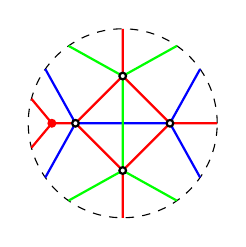
\begin{tikzpicture}[baseline=-.5ex,scale=0.6]
\draw [dashed] (0,0) circle [radius=2];
\draw[blue, thick] (145:2) -- (-1,0) -- (1,0) -- (35:2) (-145:2) -- (-1,0) (1,0) -- (-35:2);
\draw[red, thick] (165:2) -- (-1.5,0) -- (-1,0) -- (0,1) -- (0,2) (0,1)-- (1,0) -- (2,0)
(-165:2) -- (-1.5,0) (-1,0) -- (0,-1) -- (0,-2) (0,-1) -- (1,0);
\draw[green, thick](125:2) -- (0,1) -- (55:2) (-125:2) -- (0,-1) -- (-55:2) (0,-1) -- (0,1) ;
\draw[thick,red, fill=red] (-1.5,0) circle (2pt);
\draw[thick,fill=white] (-1,0) circle (2pt) (1,0) circle (2pt) (0,-1) circle (2pt) (0,1) circle (2pt);
\end{tikzpicture}
\ar[r, leftrightarrow,"\Move{II}"] & 
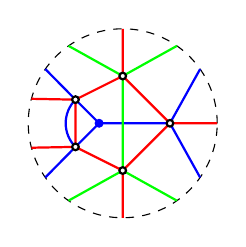
\begin{tikzpicture}[baseline=-.5ex,scale=0.6]
\draw [dashed] (0,0) circle [radius=2];
\draw[blue, thick] (145:2) -- (-1,0.5) -- (-0.5,0) -- (1,0) -- (35:2) (-145:2) -- (-1,-0.5) -- (-0.5,0) (1,0) -- (-35:2) (-1,0.5) to[out=-135,in=135] (-1,-0.5);
\draw[red, thick] (165:2) -- (-1,0.5) -- (0,1) -- (0,2) (0,1)-- (1,0) -- (2,0)
(-165:2) -- (-1,-0.5) -- (0,-1) -- (0,-2) (0,-1) -- (1,0) (-1,0.5) -- (-1,-0.5);
\draw[green, thick](125:2) -- (0,1) -- (55:2) (-125:2) -- (0,-1) -- (-55:2) (0,-1) -- (0,1) ;
\draw[thick,blue, fill=blue] (-0.5,0) circle (2pt);
\draw[thick,fill=white] (-1,0.5) circle (2pt) (-1,-0.5) circle (2pt) (1,0) circle (2pt) (0,-1) circle (2pt) (0,1) circle (2pt);
\end{tikzpicture}
\ar[rd, leftrightarrow,sloped,"\Move{VI}"]\\
& & & &
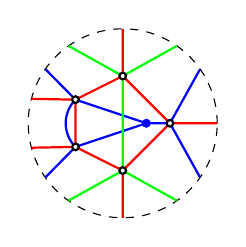
\begin{tikzpicture}[baseline=-.5ex,scale=0.6]
\draw [dashed] (0,0) circle [radius=2];
\draw[blue, thick] (145:2) -- (-1,0.5) -- (0.5,0) -- (1,0) -- (35:2) 
(-145:2) -- (-1,-0.5) -- (0.5,0) (1,0) -- (-35:2) (-1,0.5) to[out=-135,in=135] (-1,-0.5);
\draw[red, thick] (165:2) -- (-1,0.5) -- (0,1) -- (0,2) (0,1)-- (1,0) -- (2,0)
(-165:2) -- (-1,-0.5) -- (0,-1) -- (0,-2) (0,-1) -- (1,0) (-1,0.5) -- (-1,-0.5);
\draw[green, thick](125:2) -- (0,1) -- (55:2) (-125:2) -- (0,-1) -- (-55:2) (0,-1) -- (0,1) ;
\draw[thick,blue, fill=blue] (0.5,0) circle (2pt);
\draw[thick,fill=white] (-1,0.5) circle (2pt) (-1,-0.5) circle (2pt) (1,0) circle (2pt) (0,-1) circle (2pt) (0,1) circle (2pt);
\end{tikzpicture} 
\ar[dl, leftrightarrow,sloped,"\Move{II}"] \\
\begin{tikzpicture}[baseline=-.5ex,scale=1.2]
\draw [dashed] (0,0) circle [radius=1];%second circle
\clip (0,0) circle [radius=1];
\draw[rounded corners,thick, red](0,1)--(0,-1) (150:1)--++(5/4,0)--(3/4,0) (210:1)--++(5/4,0)--(3/4,0) (3/4,0)--(1,0);
\draw[Dble={green and blue},line width=2] (120:1) -- (0,0.5);
\draw[Dble={blue and green},line width=2] (60:1) -- (0,0.5);
\draw[Dble={blue and green},line width=2] (-120:1) -- (0,-0.5);
\draw[Dble={green and blue},line width=2] (-60:1) -- (0,-0.5);
\draw[blue,line width=2] (-0.05,0.5) to[out=-135,in=135] (-0.05,-0.5);
\draw[green,line width=2] (0,0.5) to[out=-135,in=135] (0,-0.5);
\draw[blue,line width=2] (0.05,0.5) to[out=-45,in=45] (0.05,-0.5);
\draw[green,line width=2] (0,0.5) to[out=-45,in=45] (0,-0.5);
\draw[thick,red,fill=red] (3/4,0) circle (1pt);
\end{tikzpicture} 
\ar[rr, "{\rm perturb}"] & &
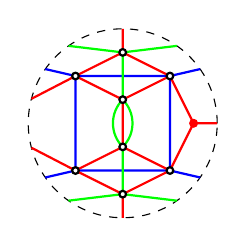
\begin{tikzpicture}[baseline=-.5ex,scale=0.6]
\draw [dashed] (0,0) circle [radius=2];
\draw[blue, thick] (145:2) -- (-1,1) -- (1,1) -- (35:2) 
(-145:2) -- (-1,-1) -- (1,-1) -- (-35:2) 
(-1,1) -- (-1,-1) (1,1) -- (1,-1);
\draw[red, thick] (165:2) -- (-1,1) -- (0,1.5) -- (0,2)
(-165:2) -- (-1,-1) -- (0,-1.5) -- (0,-2)
(0,1.5) -- (1,1) -- (1.5,0) -- (2,0)
(0,-1.5) -- (1,-1) -- (1.5,0)
(-1,1) -- (0,0.5) -- (1,1)
(-1,-1) -- (0,-0.5) -- (1,-1)
(0,0.5) -- (0,-0.5);
\draw[green, thick](125:2) -- (0,1.5) -- (55:2) 
(-125:2) -- (0,-1.5) -- (-55:2) 
(0,-1.5) -- (0,-0.5) (0,0.5) -- (0,1.5) 
(0,0.5) to[out=-135,in=135] (0,-0.5) 
(0,0.5) to[out=-45,in=45] (0,-0.5);
\draw[thick,red, fill=red] (1.5,0) circle (2pt);
\draw[thick,fill=white] (-1,1) circle (2pt) (-1,-1) circle (2pt) (1,1) circle (2pt) (1,-1) circle (2pt) (0,1.5) circle (2pt) (0,-1.5) circle (2pt) (0,0.5) circle (2pt) (0,-0.5) circle (2pt);
\end{tikzpicture} 
& 
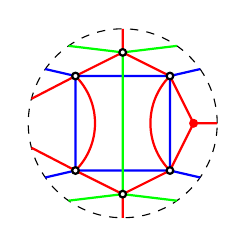
\begin{tikzpicture}[baseline=-.5ex,scale=0.6]
\draw [dashed] (0,0) circle [radius=2];
\draw[blue, thick] (145:2) -- (-1,1) -- (1,1) -- (35:2) 
(-145:2) -- (-1,-1) -- (1,-1) -- (-35:2) 
(-1,1) -- (-1,-1) (1,1) -- (1,-1);
\draw[red, thick] (165:2) -- (-1,1) -- (0,1.5) -- (0,2)
(-165:2) -- (-1,-1) -- (0,-1.5) -- (0,-2)
(0,1.5) -- (1,1) -- (1.5,0) -- (2,0)
(0,-1.5) -- (1,-1) -- (1.5,0)
(-1,1) to[out=-45, in=45] (-1,-1)
(1,1) to[out=-135, in =135] (1,-1);
\draw[green, thick](125:2) -- (0,1.5) -- (55:2) (-125:2) -- (0,-1.5) -- (-55:2) (0,-1.5) -- (0,1.5) ;
\draw[thick,red, fill=red] (1.5,0) circle (2pt);
\draw[thick,fill=white] (-1,1) circle (2pt) (-1,-1) circle (2pt) (1,1) circle (2pt) (1,-1) circle (2pt) (0,1.5) circle (2pt) (0,-1.5) circle (2pt);
\end{tikzpicture} 
\ar[from=l,leftrightarrow, "\Move{I}"] 
\end{tikzcd}
\]

\[
\begin{tikzcd}[row sep=-3pc, column sep=1pc]
\begin{tikzpicture}[baseline=-.5ex,scale=1.2]
\draw [dashed] (0,0) circle [radius=1];%first circle
\clip (0,0) circle [radius=1];
\draw[thick, red](135:1)--(-45:1) (45:1)--(-135:1);
\draw[Dble={blue and green},line width=2] (0,0) -- (-90:1);
\draw[Dble={blue and green},line width=2] (0,0) -- (90:1);
\draw[Dble={green and blue},line width=2] (0,0) -- (1,0);
\draw[Dble={green and blue},line width=2] (0,0) -- (-0.5,0);
\draw[Dble={green and blue},line width=2] (-0.5,0) -- (155:1.2);
\draw[Dble={green and blue},line width=2] (-0.5,0) -- (205:1.2);
\end{tikzpicture}
\ar[rr, "{\rm perturb.}"]\arrow[dd,"\Move{DII}"']
& &
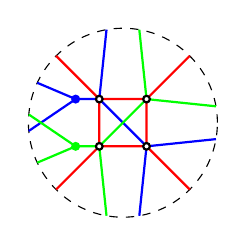
\begin{tikzpicture}[baseline=-.5ex,scale=0.6]
\draw [dashed] (0,0) circle [radius=2];
\draw[blue, thick] (155:2) -- (-1,0.5) -- (-0.5, 0.5) -- (100:2)
(-175:2) -- (-1,0.5) (-0.5, 0.5) -- (0.5,-0.5) -- (-10:2) (0.5,-0.5) -- (-80:2);
\draw[red, thick] (135:2) -- (-0.5, 0.5) -- (0.5,0.5) -- (45:2)
(-135:2) -- (-0.5, -0.5) -- (0.5,-0.5) -- (-45:2)
(-0.5,0.5) -- (-0.5,-0.5) (0.5,0.5) -- (0.5,-0.5);
\draw[green, thick] (175:2) -- (-1,-0.5) -- (-155:2) 
(-1,-0.5) -- (-0.5,-0.5) -- (0.5,0.5) -- (80:2)
(-0.5,-0.5) -- (-100:2) (0.5,0.5) -- (10:2);
\draw[thick,red, fill=red];
\draw[thick,blue, fill=blue] (-1,0.5) circle (2pt);
\draw[thick,green, fill=green] (-1,-0.5) circle (2pt);
\draw[thick,fill=white] (1/2,1/2) circle (2pt) (-1/2,1/2)circle (2pt) (1/2,-1/2)circle (2pt) (-1/2,-1/2) circle (2pt);
\end{tikzpicture}
\ar[r,leftrightarrow, "\Move{II}^2"]
&
%\begin{tikzpicture}[baseline=-.5ex,scale=0.75]
%\draw [dashed] (0,0) circle [radius=2];
%\draw[blue, thick] (155:2) -- (-1,0.5) -- (-0.5, 1) -- (100:2)
%(-175:2) -- (-1,0.5) (-0.5, 1) -- (0.5,-0.5) -- (-10:2) (0.5,-0.5) -- (-80:2);
%\draw[red, thick] (135:2) -- (-0.5, 1) -- (-0.5,0) to[out=-135,in=135] (-0.5,-1) -- (-135:2) 
%(45:2) -- (0.5,1) -- (0.5,-0.5) -- (-45:2)
%(-0.5,1) -- (0.5,1)
%(-0.5,0) -- (0,-0.5) -- (-0.5,-1)
%(0,-0.5) -- (1/2,-1/2);
%\draw[green, thick] (175:2) -- (-1/2,0) -- (-1/2,-1) -- (-155:2) (-1/2,-1) -- (-100:2)
%(80:2) -- (1/2,1) -- (10:2) (1/2,1) -- (-1/2,0);
%\draw[thick,red, fill=red] (0,-1/2) circle (2pt);
%\draw[thick,blue, fill=blue] (-1,0.5) circle (2pt);
%\draw[thick,green, fill=green] ;
%\draw[thick,fill=white] (1/2,1) circle (2pt) (-1/2,1)circle (2pt) (1/2,-1/2)circle (2pt) (-1/2,0) circle (2pt)
% (-1/2,-1) circle (2pt);
%\end{tikzpicture}
%\ar[d,leftrightarrow, "\Move{II}"]
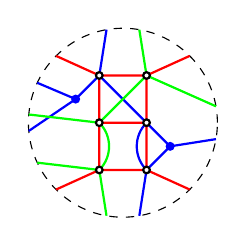
\begin{tikzpicture}[baseline=-.5ex,scale=0.6]
\draw [dashed] (0,0) circle [radius=2];
\draw[blue, thick] (155:2) -- (-1,0.5) -- (-0.5, 1) -- (100:2)
(-175:2) -- (-1,0.5) (-0.5, 1) -- (0.5,0) -- (1,-1/2) -- (-10:2) (0.5,0) to[out=-135,in=135] (0.5,-1) -- (1,-1/2) (0.5,-1) -- (-80:2);
\draw[red, thick] (135:2) -- (-0.5, 1) -- (-0.5,0) -- (-0.5,-1) -- (-135:2) 
(45:2) -- (0.5,1) -- (0.5,-1) -- (-45:2)
(-0.5,1) -- (0.5,1)
(-0.5,0) -- (0.5,0)
(-0.5,-1) -- (1/2,-1);
\draw[green, thick] (175:2) -- (-1/2,0) to[out=-45,in=45] (-1/2,-1) -- (-155:2) (-1/2,-1) -- (-100:2)
(80:2) -- (1/2,1) -- (10:2) (1/2,1) -- (-1/2,0);
\draw[thick,red, fill=red];
\draw[thick,blue, fill=blue] (-1,0.5) circle (2pt) (1,-0.5) circle (2pt);
\draw[thick,green, fill=green] ;
\draw[thick,fill=white] (-1/2,1) circle (2pt) (-1/2,0)circle (2pt) (-1/2,-1)circle (2pt) (1/2,1)circle (2pt) (1/2,0) circle (2pt) (1/2,-1) circle (2pt);
\end{tikzpicture}
\ar[rd,leftrightarrow, sloped, "\Move{IV}"]
\\
& & & &
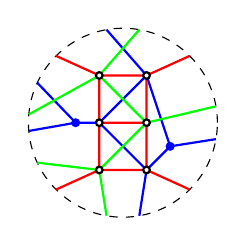
\begin{tikzpicture}[baseline=-.5ex,scale=0.6]
\draw [dashed] (0,0) circle [radius=2];
\draw[blue, thick] (155:2) -- (-1,0) -- (-0.5, 0) -- (1/2,1) -- (100:2)
(-175:2) -- (-1,0) (-1/2,0) -- (0.5,-1) -- (-80:2)
(1/2,1) -- (1,-1/2) -- (-10:2) (1/2,-1) -- (1,-1/2);
\draw[red, thick] (135:2) -- (-0.5, 1) -- (-0.5,0) -- (-0.5,-1) -- (-135:2) 
(45:2) -- (0.5,1) -- (0.5,-1) -- (-45:2)
(-0.5,1) -- (0.5,1)
(-0.5,0) -- (0.5,0)
(-0.5,-1) -- (1/2,-1);
\draw[green, thick] (175:2) -- (-1/2,1) -- (80:2)
(-155:2) -- (-1/2,-1) -- (-100:2)
(-1/2,1) -- (1/2,0) -- (-1/2,-1)  (1/2,0) -- (10:2) ;
\draw[thick,red, fill=red];
\draw[thick,blue, fill=blue] (-1,0) circle (2pt) (1,-0.5) circle (2pt);
\draw[thick,green, fill=green] ;
\draw[thick,fill=white] (-1/2,1) circle (2pt) (-1/2,0)circle (2pt) (-1/2,-1)circle (2pt) (1/2,1)circle (2pt) (1/2,0) circle (2pt) (1/2,-1) circle (2pt);
\end{tikzpicture}
\ar[dl,leftrightarrow, sloped, "\Move{II}^2"] 
\\
%\begin{tikzpicture}[baseline=-.5ex,scale=0.75]
%\draw [dashed] (0,0) circle [radius=2];
%\draw[blue, thick] (155:2) -- (-1/2,1/2) -- (0.5, 1) -- (100:2)
%(-175:2) -- (-1/2,-1/2) -- (1/2,-1) -- (-80:2)
%(-1/2,1/2) -- (-1/2, -1/2) (1/2,1) -- (1,-1/2) -- (-10:2) (1/2, -1) -- (1,-1/2);
%\draw[red, thick] (135:2) -- (-0.5,1) -- (-0.5, 1/2) to[out=-135,in=135] (-0.5,-1/2) -- (-0.5,-1) -- (-135:2) 
%(45:2) -- (0.5,1) -- (0.5,-1) -- (-45:2)
%(-0.5,1) -- (0.5,1)
%(-1/2,1/2) -- (0,0) -- (0.5,0)
%(-1/2,-1/2) -- (0,0)
%(-0.5,-1) -- (1/2,-1);
%\draw[green, thick] (175:2) -- (-1/2,1) -- (80:2)
%(-155:2) -- (-1/2,-1) -- (-100:2)
%(-1/2,1) -- (1/2,0) -- (-1/2,-1)  (1/2,0) -- (10:2) ;
%\draw[thick,red, fill=red] (0,0) circle (2pt) ;
%\draw[thick,blue, fill=blue] (1,-0.5) circle (2pt);
%\draw[thick,green, fill=green] ;
%\draw[thick,fill=white] (-1/2,1) circle (2pt) (-1/2,1/2)circle (2pt) (-1/2,-1/2)circle (2pt) (-1/2,-1)circle (2pt) (1/2,1)circle (2pt) (1/2,0) circle (2pt) (1/2,-1) circle (2pt);
%\end{tikzpicture} 
%\ar[d,leftrightarrow, "\Move{II}"]
\begin{tikzpicture}[baseline=-.5ex,scale=1.2]
\draw [dashed] (0,0) circle [radius=1];%second circle
\clip (0,0) circle [radius=1];
\draw[thick, red](120:1)--(0,0.5) to[out=-45,in=45] (0,-0.5) --(-120:1)
(60:1)--(0,0.5) to[out=-135,in=135] (0,-0.5) --(-60:1);
\draw[Dble={green and blue},line width=2] (0,0.5) -- ++(-1,0);
\draw[Dble={green and blue},line width=2] (0,0.5) -- (0.3,0.5);
\draw[Dble={green and blue},line width=2] (0,1) -- (0,0.5);
\draw[Dble={green and blue},line width=2] (0,0) -- (0,0.5);
\draw[Dble={green and blue},line width=2] (0,0) -- (0,-0.5);
\draw[Dble={green and blue},line width=2] (0,-0.5) -- ++(-1,0);
\draw[Dble={green and blue},line width=2] (0,-0.5) -- (0.3,-0.5);
\draw[Dble={green and blue},line width=2] (0,-1) -- (0,-0.5);
\draw[blue,line width=2]
(0.3,-0.525) to[out=0,in=-135] (0.7,-0.025) 
(0.3,0.475) to[out=0,in=135] (0.7,-0.025) -- (1,-0.025);
\draw[green,line width=2]
(0.3,-0.475) to[out=0,in=-135] (0.7,0.025) 
(0.3,0.525) to[out=0,in=135] (0.7,0.025) -- (1,0.025);
\end{tikzpicture}
\ar[rr, "{\rm perturb.}"] 
& &
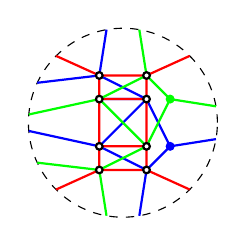
\begin{tikzpicture}[baseline=-.5ex,scale=0.6]
\draw [dashed] (0,0) circle [radius=2];
\draw[blue, thick] (155:2) -- (-1/2,1) -- (100:2)
(-175:2) -- (-1/2,-1/2) -- (1/2,-1) -- (-80:2)
(-1/2,1/2) -- (1/2, 1/2) -- (-1/2,-1/2) (1/2,1/2) -- (1,-1/2) -- (-10:2) (1/2, -1) -- (1,-1/2)
(-1/2, 1) -- (1/2, 1/2)
;
\draw[red, thick] (135:2) -- (-0.5,1) -- (-0.5,-1) -- (-135:2) 
(45:2) -- (0.5,1) -- (0.5,-1) -- (-45:2)
(-0.5,1) -- (0.5,1)
(-1/2,1/2) -- (0.5,1/2)
(-1/2,-1/2) -- (1/2,-1/2)
(-0.5,-1) -- (1/2,-1);
\draw[green, thick] (175:2) -- (-1/2,1/2) -- (1/2,1) -- (80:2)
(-155:2) -- (-1/2,-1) -- (-100:2)
(-1/2,1/2) -- (1/2,-1/2) -- (-1/2,-1)
(1/2,1) -- (1,1/2) -- (1/2,-1/2)
(1,1/2) -- (10:2);
\draw[thick,blue, fill=blue] (1,-0.5) circle (2pt);
\draw[thick,red, fill=red] ;
\draw[thick,green, fill=green](1,1/2) circle (2pt) ;
\draw[thick,fill=white] (-1/2,1) circle (2pt) (-1/2,1/2)circle (2pt) (-1/2,-1/2)circle (2pt) (-1/2,-1)circle (2pt) (1/2,1)circle (2pt) (1/2,1/2) circle (2pt) (1/2,-1/2) circle (2pt)  (1/2,-1) circle (2pt);
\end{tikzpicture} 
\ar[r,leftrightarrow, "\Move{IV}"] 
&
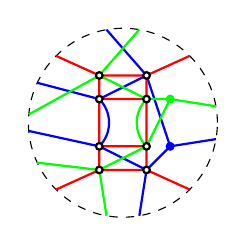
\begin{tikzpicture}[baseline=-.5ex,scale=0.6]
\draw [dashed] (0,0) circle [radius=2];
\draw[blue, thick] (155:2) -- (-1/2,1/2) -- (0.5, 1) -- (100:2)
(-175:2) -- (-1/2,-1/2) -- (1/2,-1) -- (-80:2)
(-1/2,1/2) to[out=-45,in=45] (-1/2, -1/2) (1/2,1) -- (1,-1/2) -- (-10:2) (1/2, -1) -- (1,-1/2);
\draw[red, thick] (135:2) -- (-0.5,1) -- (-0.5,-1) -- (-135:2) 
(45:2) -- (0.5,1) -- (0.5,-1) -- (-45:2)
(-0.5,1) -- (0.5,1)
(-1/2,1/2) -- (0.5,1/2)
(-1/2,-1/2) -- (1/2,-1/2)
(-0.5,-1) -- (1/2,-1);
\draw[green, thick] (175:2) -- (-1/2,1) -- (80:2)
(-155:2) -- (-1/2,-1) -- (-100:2)
(-1/2,1) -- (1/2,1/2) to[out=-135,in=135] (1/2,-1/2) -- (-1/2,-1)
(1/2,1/2) -- (1,1/2) -- (10:2)
(1/2,-1/2) -- (1,1/2);
\draw[thick,red, fill=red] ;
\draw[thick,blue, fill=blue] (1,-0.5) circle (2pt);
\draw[thick,green, fill=green](1,1/2) circle (2pt) ;
\draw[thick,fill=white] (-1/2,1) circle (2pt) (-1/2,1/2)circle (2pt) (-1/2,-1/2)circle (2pt) (-1/2,-1)circle (2pt) (1/2,1)circle (2pt) (1/2,1/2) circle (2pt) (1/2,-1/2) circle (2pt)  (1/2,-1) circle (2pt);
\end{tikzpicture} 
\end{tikzcd}
\]


\subsection{Justifications of Legendrian local mutations in degenerate $N$-graphs}\label{appendix:local mutations}
\[
\begin{tikzcd}[row sep=-3pc]
\begin{tikzpicture}[baseline=-.5ex, scale=0.4]
\draw[red] (-2,0) node[above] {$\cycle$};
\draw[dashed] (0,0) circle (3);
\draw[color=cyclecolor2, opacity=0.5, line width=5] (-3,0) -- (3,0);
\draw[thick, red] (-3,0) -- (3,0) (0,-3) -- (0,3);
\draw[Dble={green and blue},line width=2] (0,0) -- (45:3);
\draw[Dble={green and blue},line width=2] (135:3) -- (0,0);
\draw[Dble={green and blue},line width=2] (0,0) -- (-135:3);
\draw[Dble={green and blue},line width=2] (-45:3) -- (0,0);
\end{tikzpicture}
\arrow[r, "\text{Perturb}"]\arrow[dd,"\mutation_\cycle"'] &
\begin{tikzpicture}[baseline=-.5ex, scale=0.4]
\draw[dashed] (0,0) circle (3);
\clip (0,0) circle (3);
\draw[color=cyclecolor2, opacity=0.5, line width=5] (-3,0) -- (3,0);
\draw[red, thick] (-3,0) -- (-1,0) -- (0,1) -- (1,0) -- (0,-1) -- (-1,0) (1,0) -- (3,0) (0,1) -- (0,3) (0,-1) -- (0,-3);
\draw[blue, thick] (-1,0) -- +(135:3) ++(0,0) -- +(-135:3) (1,0) -- +(45:3) ++(0,0) -- +(-45:3) (-1,0) -- (1,0);
\draw[green, thick] (0,1) -- +(135:3) ++(0,0) -- +(45:3) (0,-1) -- +(-135:3) ++(0,0) -- +(-45:3) (0,-1) -- (0,1);
\draw[thick, fill=white] (-1,0) circle (0.1) (0,1) circle (0.1) (1,0) circle (0.1) (0,-1) circle (0.1);
\end{tikzpicture}
\arrow[rd, sloped, "\mutation_\cycle"]\\
& &
\begin{tikzpicture}[baseline=-.5ex, scale=0.4]
\draw[dashed] (0,0) circle (3);
\clip (0,0) circle (3);
\draw[color=cyclecolor2, opacity=0.5, line width=5] (-3,0) -- (3,0);
\draw[blue, thick] (1,1.5) to[out=-60,in=60] (1,0) to[out=-60,in=60] (1,-1.5) 
(-1,-1.5) to[out=120,in=-120] (-1,0) to[out=120,in=-120] (-1,1.5);
\draw[red, thick] (0,2) -- (-1,1.5) to[out=-60,in=60] (-1,0) to[out=-60,in=60] (-1,-1.5) -- (0,-2) -- (1,-1.5) to[out=120,in=-120] (1,0) to[out=120,in=-120] (1,1.5) -- cycle;
\draw[red, thick] (-3,0) -- (-1,0) (1,0) -- (3,0);
\draw[blue, thick] (-1,0) --(1,0);
\begin{scope}[yshift=1.5cm]
\draw[red, thick] (-3,0) -- (-1,0) (1,0) -- (3,0);
\draw[blue, thick] (-1,0) --(1,0);
\end{scope}
\begin{scope}[yshift=-1.5cm]
\draw[red, thick] (-3,0) -- (-1,0) (1,0) -- (3,0);
\draw[blue, thick] (-1,0) --(1,0);
\end{scope}
\draw[blue, thick] (-1,1.5) -- +(135:3) (-1,-1.5) -- +(-135:3) (1,1.5) -- +(45:3) (1,-1.5) -- +(-45:3);
\draw[green, thick] (0,2) -- +(135:3) ++(0,0) -- +(45:3) (0,-2) -- +(-135:3) ++(0,0) -- +(-45:3) (0,-2) -- (0,2);
\draw[thick, fill=white] (-1,0) circle (0.1) (-1,1.5) circle (0.1) (-1,-1.5) circle (0.1) (0,2) circle (0.1) (1,0) circle (0.1) (1,1.5) circle (0.1) (1,-1.5) circle (0.1) (0,-2) circle (0.1);
\end{tikzpicture}
\arrow[dl, leftrightarrow, sloped, "\Move{I}^2"]\\
\begin{tikzpicture}[baseline=-.5ex, scale=0.4]
\draw[red] (2,0) node[above] {$\cycle'$};
\draw[dashed] (0,0) circle (3);
\clip (0,0) circle (3);
\draw[color=cyclecolor2, opacity=0.5, line width=5] (-3,0) -- (3,0);
\draw[thick, red] (-3,0) -- (3,0) (-3,1) -- (3,1) (-3,-1) -- (3,-1) (0,-3) -- (0,3);
\draw[Dble={green and blue},line width=2] (0,1) -- (45:3);
\draw[Dble={green and blue},line width=2] (135:3) -- (0,1);
\draw[Dble={green and blue},line width=2] (0,-1) -- (-135:3);
\draw[Dble={green and blue},line width=2] (-45:3) -- (0,-1);
\draw[blue,line width=2] 
(-0.1,1) to[out=-180,in=180] (-0.1,0) 
(0.1,1) to[out=0,in=0] (0.1,0)
(-0.1,-1) to[out=-180,in=180] (-0.1,0) 
(0.1,-1) to[out=0,in=0] (0.1,0);
\draw[green,line width=2] 
(0,0.95) to[out=-180,in=180] (0,0.05)
(0,0.95) to[out=0,in=0] (0,0.05)
(0,-0.95) to[out=-180,in=180] (0,-0.05)
(0,-0.95) to[out=0,in=0] (0,-0.05);
\end{tikzpicture}
\arrow[r,"\text{Perturb}"']
&
\begin{tikzpicture}[baseline=-.5ex, scale=0.4]
\draw[dashed] (0,0) circle (3);
\clip (0,0) circle (3);
\draw[color=cyclecolor2, opacity=0.5, line width=5] (-3,0) -- (3,0);
\draw[blue, thick] (1,1.5) to[out=-60,in=60] (1,0) to[out=-60,in=60] (1,-1.5) 
(-1,-1.5) to[out=120,in=-120] (-1,0) to[out=120,in=-120] (-1,1.5);
\draw[red, thick] (0,2) -- (-1,1.5) -- (0,1) (0, 0.5) -- (-1,0) -- (0,-0.5) (0,-1) -- (-1,-1.5) -- (0,-2) -- (1,-1.5) -- (0, -1) (0, -0.5) -- (1,0) -- (0, 0.5) (0,1) -- (1,1.5) -- (0,2) (0,1) -- (0,0.5) (0,-1) -- (0,-0.5);
\draw[red, thick] (-3,0) -- (-1,0) (1,0) -- (3,0);
\draw[blue, thick] (-1,0) --(1,0);
\begin{scope}[yshift=1.5cm]
\draw[red, thick] (-3,0) -- (-1,0) (1,0) -- (3,0);
\draw[blue, thick] (-1,0) --(1,0);
\end{scope}
\begin{scope}[yshift=-1.5cm]
\draw[red, thick] (-3,0) -- (-1,0) (1,0) -- (3,0);
\draw[blue, thick] (-1,0) --(1,0);
\end{scope}
\draw[blue, thick] (-1,1.5) -- +(135:3) (-1,-1.5) -- +(-135:3) (1,1.5) -- +(45:3) (1,-1.5) -- +(-45:3);
\draw[green, thick] (0,2) -- +(135:3) ++(0,0) -- +(45:3) (0,-2) -- +(-135:3) ++(0,0) -- +(-45:3) (0,2) -- (0,1) (0,0.5) -- (0,-0.5) (0,-1) -- (0,-2) (0, 0.75) circle (0.25) (0, -0.75) circle (0.25);
\draw[thick, fill=white] (-1,0) circle (0.1) (-1,1.5) circle (0.1) (-1,-1.5) circle (0.1) (0,2) circle (0.1) (1,0) circle (0.1) (1,1.5) circle (0.1) (1,-1.5) circle (0.1) (0,-2) circle (0.1) (0,0.5) circle (0.1) (0,1) circle (0.1) (0,-0.5) circle (0.1) (0,-1) circle (0.1);
\end{tikzpicture}
\end{tikzcd}
\]

\[
\begin{tikzcd}[row sep=1pc, column sep=1pc]
\begin{tikzpicture}[baseline=-.5ex, scale=0.4]
\draw[dashed] (0,0) circle (3);
\clip (0,0) circle (3);
\draw[color=blue!50!green!50] (-2,0) node[above] {$\cycle_I$};
\draw[thick, red] (45:3) -- (-135:3) (135:3) -- (-45:3);
\draw[Dble={blue and green},line width=2] (-3,0) -- (0,0);
\draw[Dble={blue and green},line width=2] (3,0) -- (0,0);
\draw[Dble={blue and green},line width=2] (0,0) --(0,3);
\draw[Dble={blue and green},line width=2] (0,0) -- (0,-3);
\draw[color=cyclecolor1, opacity=0.5, line width=7] (-3,0) -- (3,0);
\end{tikzpicture}
\arrow[rr,"\text{Perturb}"]\arrow[d, "
\mutation_{\cycle_I}"']&&
\begin{tikzpicture}[baseline=-.5ex, scale=0.4]
\draw[dashed] (0,0) circle (3);
\clip (0,0) circle (3);
\draw[color=cyclecolor1, opacity=0.5, line width=7] (-3,0.707) -- (3,0.707);
\draw[color=cyclecolor1, opacity=0.5, line width=7] (-3,-0.707) -- (3,-0.707);
\draw[red, thick] (45:1) -- (45:3) (-45:1) -- (-45:3) (45:-1) -- (45:-3) (-45:-1) -- (-45:-3) (45:-1) rectangle (45:1);
\draw[blue, thick] (-45:1) -- +(3,0) +(0,0) -- ++(0,-3) (-45:-1) -- +(-3,0) +(0,0) -- ++(0,3) (-45:1) -- (-45:-1);
\draw[green, thick] (45:1) -- +(3,0) +(0,0) -- ++(0,3) (45:-1) -- +(-3,0) +(0,0) -- ++(0,-3) (45:1) -- (45:-1);
\draw[thick, fill=white] (45:1) circle (0.1) (45:-1) circle (0.1) (-45:1) circle (0.1) (-45:-1) circle (0.1);
\end{tikzpicture}
\arrow[r, "\mutation_{\cycle_I}"]&
\begin{tikzpicture}[baseline=-.5ex, scale=0.4]
\draw[dashed] (0,0) circle (3);
\clip (0,0) circle (3);
\draw[color=cyclecolor1, opacity=0.5, line width=7] (-3,1.2) -- (3,1.2) (-3, -1.2) -- (3, -1.2);
\draw[thick, blue] (-3, 2) -- (-1, 2) (1, -2) -- (3, -2)
(-3, 1.2) -- (-1, 1.2) (1, -1.2) -- (3, -1.2)
(-3, 0.4) -- (-1, 0.4) (1, -0.4) -- (3, -0.4)
(-1, 2) -- (-1,3) (1,-2) -- (1,-3)
(-1, 2) to[out=-30, in=30] (-1, 1.2) to[out=-30, in=30] (-1, 0.4) -- (1, -0.4) to[out=-150, in=150] (1, -1.2) to[out=-150, in=150] (1, -2)
;
\draw[thick, green] (-3,-2) -- (-1, -2) (1, 2) -- (3, 2)
(-3, -1.2) -- (-1, -1.2) (1, 1.2) -- (3, 1.2)
(-3, -0.4) -- (-1, -0.4) (1, 0.4) -- (3, 0.4)
(1, 2) -- (1,3) (-1,-2) -- (-1,-3)
(1, 2) to[out=-150, in=150] (1, 1.2) to[out=-150, in=150] (1, 0.4) -- (-1, -0.4) to[out=-30, in=30] (-1, -1.2) to[out=-30, in=30] (-1, -2)
;
\draw[thick, red] 
(-1, 2) -- (-1, -2) (1, 2) -- (1, -2)
(-1, 2) -- ++(-45:-1) (1, 2) -- ++(45:1) (-1, -2) -- ++(45:-1) (1,-2) -- ++(-45:1);
\foreach \y in {-2, -1.2, -0.4, 0.4, 1.2, 2} {
\draw[thick, red] (-1, \y) -- (1, \y);
\draw[thick, fill=white] (-1, \y) circle (0.1) (1,\y) circle (0.1);
}
\end{tikzpicture}
\arrow[d, leftrightarrow, "\Move{IV}"]
\\
\begin{tikzpicture}[baseline=-.5ex, scale=0.4]
\draw[dashed] (0,0) circle (3);
\clip (0,0) circle (3);
\draw[thick, red, rounded corners] 
(45:3) -- (0,1) -- (-0.5, 0.5) -- (0.5, -0.5) -- (0,-1) -- (-135:3)
(-45:3) -- (0,-1) -- (-0.5, -0.5) -- (0.5, 0.5) -- (0,1) -- (135:3);
\draw[Dble={green and blue},line width=2] (0,3) --(0,1);
\draw[Dble={green and blue},line width=2] (0,0.5) --(0,0);
\draw[Dble={green and blue},line width=2] (0,-0.5) --(0,-1);
\draw[Dble={green and blue},line width=2] (0,-3) -- (0,-1);
\draw[Dble={green and blue},line width=2] (0,-0.5) --(0,0);
\draw[Dble={green and blue},line width=2] (0,0.5) -- (0,1);
\begin{scope}
\draw[Dble={green and blue},line width=2] (0,0) -- (-3,0);
\draw[Dble={green and blue},line width=2] (0,0) -- (3,0);
\draw[color=cyclecolor1, opacity=0.5, line width=7] (-3,0) -- (3,0);
\end{scope}
\begin{scope}[yshift=-1cm]
\draw[Dble={green and blue},line width=2] (0,0) -- (-3,0);
\draw[Dble={green and blue},line width=2] (0,0) -- (3,0);
\end{scope}
\begin{scope}[yshift=1cm]
\draw[Dble={green and blue},line width=2] (0,0) -- (-3,0);
\draw[Dble={green and blue},line width=2] (0,0) -- (3,0);
\end{scope}
\draw[color=blue!50!green!50] (2,0) node[above] {$\cycle'_I$};
\end{tikzpicture}
\arrow[rr,"\text{Perturb}"']
&&
\begin{tikzpicture}[baseline=-.5ex, scale=0.4]
\draw[dashed] (0,0) circle (3);
\clip (0,0) circle (3);
\draw[color=cyclecolor1, opacity=0.5, line width=7] (-3,0.4) -- (3,0.4) (-3, -0.4) -- (3, -0.4);
\draw[thick, blue] (-3, 2) -- (-1, 2) (1, -2) -- (3, -2)
(-3, -1.2) -- (-1, -1.2) (1, 1.2) -- (3, 1.2)
(-3, 0.4) -- (-1, 0.4) (1, -0.4) -- (3, -0.4)
(-1, 2) -- (-1,3) (1,-2) -- (1,-3)
(-1, 2) -- (1, 1.2) -- (-1, 0.4) -- (1, -0.4) -- (-1, -1.2) -- (1, -2)
;
\draw[thick, green] (-3,-2) -- (-1, -2) (1, 2) -- (3, 2)
(-3, 1.2) -- (-1, 1.2) (1, -1.2) -- (3, -1.2)
(-3, -0.4) -- (-1, -0.4) (1, 0.4) -- (3, 0.4)
(1, 2) -- (1,3) (-1,-2) -- (-1,-3)
(1, 2) -- (-1, 1.2) -- (1, 0.4) -- (-1, -0.4) -- (1, -1.2) -- (-1, -2)
;
\draw[thick, red] 
(-1, 2) -- (-1, -2) (1, 2) -- (1, -2)
(-1, 2) -- ++(-45:-1) (1, 2) -- ++(45:1) (-1, -2) -- ++(45:-1) (1,-2) -- ++(-45:1);
\foreach \y in {-2, -1.2, -0.4, 0.4, 1.2, 2} {
\draw[thick, red] (-1, \y) -- (1, \y);
\draw[thick, fill=white] (-1, \y) circle (0.1) (1,\y) circle (0.1);
}
\end{tikzpicture}
\arrow[r, leftrightarrow, "\Move{IV}^2"]
&
\begin{tikzpicture}[baseline=-.5ex, scale=0.4]
\draw[dashed] (0,0) circle (3);
\clip (0,0) circle (3);
\draw[color=cyclecolor1, opacity=0.5, line width=7] (-3,1.2) -- (3,1.2) (-3, -1.2) -- (3, -1.2);
\draw[thick, blue] (-3, 2) -- (-1, 2) (1, -2) -- (3, -2)
(-3, 1.2) -- (-1, 1.2) (1, -1.2) -- (3, -1.2)
(-3, -0.4) -- (-1, -0.4) (1, 0.4) -- (3, 0.4)
(-1, 2) -- (-1,3) (1,-2) -- (1,-3)
(-1, 2) to[out=-30, in=30] (-1, 1.2) -- (1, 0.4) -- (-1, -0.4) -- (1, -1.2) to[out=-150, in=150] (1, -2)
;
\draw[thick, green] (-3,-2) -- (-1, -2) (1, 2) -- (3, 2)
(-3, -1.2) -- (-1, -1.2) (1, 1.2) -- (3, 1.2)
(-3, 0.4) -- (-1, 0.4) (1, -0.4) -- (3, -0.4)
(1, 2) -- (1,3) (-1,-2) -- (-1,-3)
(1, 2) to[out=-150, in=150] (1, 1.2) -- (-1, 0.4) -- (1, -0.4) -- (-1, -1.2) to[out=-30, in=30] (-1, -2)
;
\draw[thick, red] 
(-1, 2) -- (-1, -2) (1, 2) -- (1, -2)
(-1, 2) -- ++(-45:-1) (1, 2) -- ++(45:1) (-1, -2) -- ++(45:-1) (1,-2) -- ++(-45:1);
\foreach \y in {-2, -1.2, -0.4, 0.4, 1.2, 2} {
\draw[thick, red] (-1, \y) -- (1, \y);
\draw[thick, fill=white] (-1, \y) circle (0.1) (1,\y) circle (0.1);
}
\end{tikzpicture}
\end{tikzcd}
\]

\subsection{Equivalence between $\ngraph(1,b,c)$ and a stabilization of $\ngraph(\dynA_n)$}
\label{appendix:tripod with a=1 is of type An}

A stabilization of $\ngraph(\dynA_n)$ is a $3$-graph which is $\boundary$-Legendrian isotopic to a $3$-graph $S(\ngraph(\dynA_n))$ given as follows:
\[
\begin{tikzcd}
\ngraph(\dynA_n)=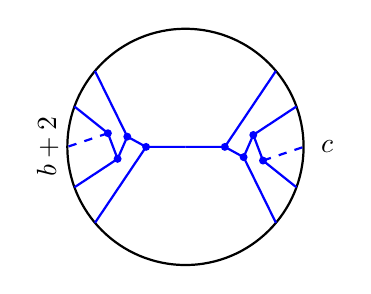
\begin{tikzpicture}[baseline=-.5ex,xscale=0.5, yscale=0.5]
\draw[thick] (0,0) circle (3cm);
\foreach \i in {120,300} {
\draw[blue, thick, fill] (0,0) -- (60+\i:1) circle (2pt) -- (100+\i:3) (60+\i:1) -- (50+\i:1.5) circle (2pt) -- (20+\i:3) (50+\i:1.5) -- (70+\i:1.75) circle (2pt) -- (80+\i:3) (70+\i:1.75) -- (50+\i:2) circle (2pt) -- (40+\i:3);
\draw[blue, thick, dashed] (50+\i:2) -- (60+\i:3);
}
\curlybrace[]{135}{225}{3.2};
\draw (180:3.5) node[rotate=90] {$b+2$};
\curlybrace[]{315}{405}{3.2};
\draw (0:3.2) node[right] {$c$};
\end{tikzpicture}
\arrow[r,"\Move{S}"]&
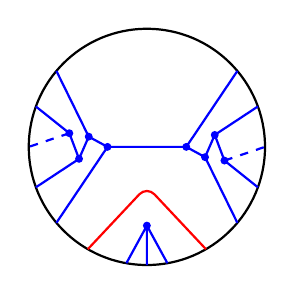
\begin{tikzpicture}[baseline=-.5ex,xscale=0.5,yscale=0.5]
\draw[thick] (0,0) circle (3cm);
\foreach \i in {120,300} {
\draw[blue, thick, fill] (0,0) -- (60+\i:1) circle (2pt) -- (100+\i:3) (60+\i:1) -- (50+\i:1.5) circle (2pt) -- (20+\i:3) (50+\i:1.5) -- (70+\i:1.75) circle (2pt) -- (80+\i:3) (70+\i:1.75) -- (50+\i:2) circle (2pt) -- (40+\i:3);
\draw[blue, thick, dashed] (50+\i:2) -- (60+\i:3);
}
\draw[red, thick, rounded corners] (240:3) -- (270:1) -- (300:3);
\draw[blue, thick] (260:3) -- (270:2) -- (280:3) (270:3) -- (270:2);
\draw[blue, thick, fill] (270:2) circle (2pt);
\end{tikzpicture}
=S(\ngraph(\dynA_n))
\end{tikzcd}
\]

Now we attach the annular $3$-graph corresponding to Legendrian isotopy from $S(\beta(\dynA_n))$ to~$\beta(1,b,c)$ given above.
Then we have the following $3$-graph which is $\boundary$-Legendrian isotopic to~$S(\ngraph(\dynA_n))$.
\[
\begin{tikzcd}[column sep=5pc]
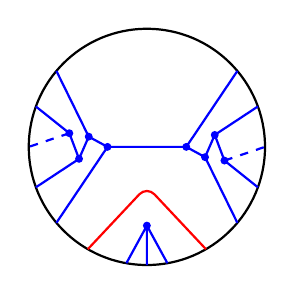
\begin{tikzpicture}[baseline=-.5ex,xscale=0.5,yscale=0.5]
\draw[thick] (0,0) circle (3cm);
\foreach \i in {120,300} {
\draw[blue, thick, fill] (0,0) -- (60+\i:1) circle (2pt) -- (100+\i:3) (60+\i:1) -- (50+\i:1.5) circle (2pt) -- (20+\i:3) (50+\i:1.5) -- (70+\i:1.75) circle (2pt) -- (80+\i:3) (70+\i:1.75) -- (50+\i:2) circle (2pt) -- (40+\i:3);
\draw[blue, thick, dashed] (50+\i:2) -- (60+\i:3);
}
\draw[red, thick, rounded corners] (240:3) -- (270:1) -- (300:3);
\draw[blue, thick] (260:3) -- (270:2) -- (280:3) (270:3) -- (270:2);
\draw[blue, thick, fill] (270:2) circle (2pt);
\end{tikzpicture}
\arrow[r,"\boundary\text{-Legendrian}","\text{isotopic}"']&
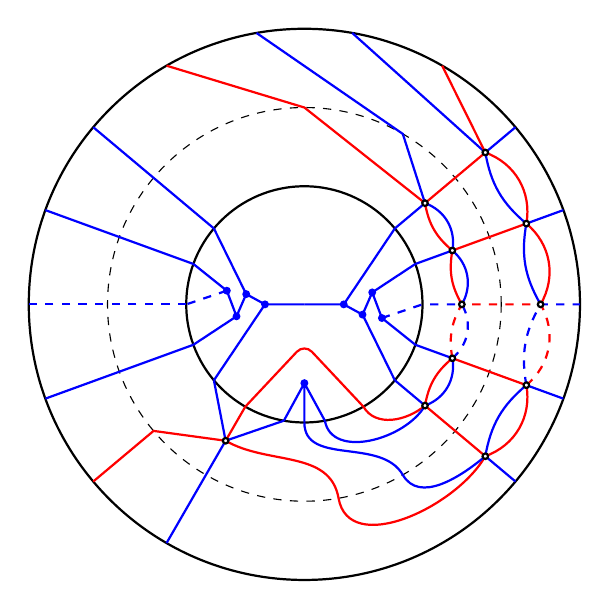
\begin{tikzpicture}[baseline=-.5ex,xscale=0.5,yscale=0.5]
\draw[thick](0,0) circle (7cm) (0,0) circle (3cm);
\draw[dashed] (0,0) circle (5cm);
\foreach \i in {120,300} {
\draw[blue, thick, fill] (0,0) -- (60+\i:1) circle (2pt) -- (100+\i:3) (60+\i:1) -- (50+\i:1.5) circle (2pt) -- (20+\i:3) (50+\i:1.5) -- (70+\i:1.75) circle (2pt) -- (80+\i:3) (70+\i:1.75) -- (50+\i:2) circle (2pt) -- (40+\i:3);
\draw[blue, thick, dashed] (50+\i:2) -- (60+\i:3);
}
\draw[red, thick, rounded corners] (240:3) -- (270:1) -- (300:3);
\draw[blue, thick] (260:3) -- (270:2) -- (280:3) (270:3) -- (270:2);
\draw[blue, thick, fill] (270:2) circle (2pt);
%
\draw[red, thick] (240:3) -- (240:4) -- (220:5) -- (220:7) (240:4) to[out=330,in=100] (280:5) to[out=280,in=240] (320:6);
\draw[blue, thick] (220:3) -- (240:4) (260:3) -- (240:4) (240:4) -- (240:7);
%
\draw[blue, thick] (270:3) to[out=270,in=120] (300:5) to[out=300,in=220] (320:6) -- (320:7);
%
\draw[red, thick] (300:3) to[out=300,in=220] (320:4);
\draw[blue, thick] (280:3) to[out=280,in=240] (320:4);
%
\foreach \r in {140, 160, 200} {
\begin{scope}[rotate=\r]
\draw[blue, thick] (0:3) -- (0:7);
\end{scope}
}
\draw[blue, thick, dashed] (180:3) -- (180:7);
%
\foreach \r in {320, 0, 20} {
\begin{scope}[rotate=\r]
\draw[red, thick] (0:4) to[out=120,in=-100] (20:4) -- (20:6);
\draw[blue, thick] (0:4) to[out=60, in=-40] (20:4) -- (20:3);
\draw[blue, thick] (0:6) to[out=120,in=-100] (20:6) -- (20:7);
\draw[red, thick] (0:6) to[out=60, in=-40] (20:6);
\end{scope}
}
\begin{scope}[rotate=340, dashed]
\draw[red, thick] (0:4) to[out=120,in=-100] (20:4) -- (20:6);
\draw[blue, thick] (0:4) to[out=60, in=-40] (20:4) -- (20:3);
\draw[blue, thick] (0:6) to[out=120,in=-100] (20:6) -- (20:7);
\draw[red, thick] (0:6) to[out=60, in=-40] (20:6);
\end{scope}
\draw[red, thick] (320:4) -- (320:6);
\draw[blue, thick] (320:4) -- (320:3);
%
\draw[red, thick] (40:4) -- (90:5) -- (120:7);
\draw[blue, thick] (40:4) -- (60:5) -- (100:7);
\draw[blue, thick] (40:6) -- (80:7);
\draw[red, thick] (40:6) -- (60:7);
%
\foreach \r in {320, 340, 360, 380, 400} {
\begin{scope}[rotate=\r]
\draw[thick, fill=white] (0:4) circle (2pt);
\draw[thick, fill=white] (0:6) circle (2pt);
\end{scope}
}
\draw[thick, fill=white] (240:4) circle (2pt);
\end{tikzpicture}
\end{tikzcd}
\]
%
%the second picture in Figure~\ref{figure:proof of stabilization}.
%Then by adding an annular $N$-graph corresponding to a sequence of $\Move{RIII}$, we obtain the third, which is $\boundary$-Legendrian isotopic to $S(\ngraph(\dynA_n))$ and produces the fourth by applying the following generalized push-through move.
By applying the following generalized push-through move,
\[
\begin{tikzcd}
\begin{tikzpicture}[baseline=-.5ex,scale=0.6]
\draw[dashed] \boundellipse{0.75,0}{3}{2};
\draw[blue, thick](-1.2,1.5) -- (0,1.5) (-2.15,0.5) -- (0,0.5) (-2.15,-0.5) -- (0,-0.5) (-1.2,-1.5) -- (0,-1.5);
\draw[blue, thick] (0.5,2) --  (0,1.5) to[out=-60,in=60] (0,0.5) to[out=-60,in=100] (0.1,0.2) (0.1,-0.2) to[out=-100,in=60] (0,-0.5) to[out=-60,in=60] (0,-1.5) -- (0.5,-2);
\draw[blue, thick, densely dotted] (0.1, 0.2) -- (0.1, -0.2);
\draw[red, thick] (-0.35,1.85) --  (0,1.5) to[out=-120,in=120] (0,0.5) to[out=-120,in=80] (-0.1,0.2) (-0.1,-0.2) to[out=-80,in=120] (0,-0.5) to[out=-120,in=120] (0,-1.5) -- (-0.35,-1.85);
\draw[red, thick, densely dotted] (-0.1, 0.2) -- (-0.1, -0.2);
\draw[red, thick, fill] (3.75,0) -- (2.5,0) circle (2pt) -- (0,-1.5) (2.5,0) -- (2, 0.5) circle (2pt) -- (0,1.5) (2,0.5) -- (1.5,0) circle (2pt) -- (0,-0.5) (1.5,0) -- (1, 0.5) circle (2pt) -- (0,0.5);
\draw[red, thick, dashed] (1,0.5) -- (0.5,0);
\draw[fill=white, thick] (0,1.5) circle (2pt) (0,0.5) circle (2pt) (0,-0.5) circle (2pt) (0,-1.5) circle (2pt);
\end{tikzpicture}
\arrow[leftrightarrow, r,"\Move{II^*}"]&
\begin{tikzpicture}[baseline=-.5ex,scale=0.6]
\draw[dashed] \boundellipse{1.7,0}{2.5}{2};
\draw[blue, thick, fill] (3,0) -- (2.5,0) circle (2pt) -- (0,-1.5) (2.5,0) -- (2, 0.5) circle (2pt) -- (0,1.5) (2,0.5) -- (1.5,0) circle (2pt) -- (-0.75,-0.5) (1.5,0) -- (1, 0.5) circle (2pt) -- (-0.75,0.5);
\draw[blue, thick, dashed] (1,0.5) -- (0.5,0);
\draw[blue, thick] (3.4,1.5) -- (3,0) -- (3.4,-1.5);
\draw[red, thick] (2.5,1.9) -- (3,0) -- (2.5,-1.9) (3,0) -- (4.2,0);
\draw[fill=white, thick] (3,0) circle (2pt);
\end{tikzpicture}
\end{tikzcd}
\]
we obtain the $3$-graph in the left of the following three equivalent $3$-graphs
\[
\begin{tikzcd}[column sep=1.5pc]
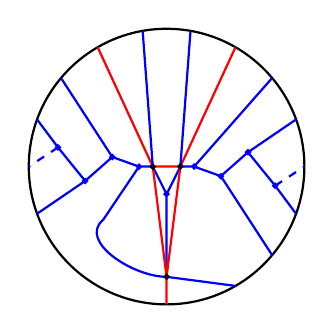
\begin{tikzpicture}[baseline=-.5ex,xscale=0.35,yscale=0.35]
\draw[thick] (0,0) circle (5cm);
\draw[blue, thick, fill] (-0.5,0) -- (-1,0) circle (2pt) -- (220:3) (-1,0) -- (170:2) circle (2pt) -- (140:5) (170:2) -- (190:3) circle (2pt) -- (200:5) (190:3) -- (170:4) circle (2pt) -- (160:5);
\draw[blue, thick, dashed] (170:4) -- (180:5);
%
\draw[blue, thick, fill] (0.5,0) -- (1,0) circle (2pt) -- (40:5) (1,0) -- (-10:2) circle (2pt) -- (-40:5) (-10:2) -- (10:3) circle (2pt) -- (20:5) (10:3) -- (-10:4) circle (2pt) -- (-20:5);
\draw[blue, thick, dashed] (-10:4) -- (0:5);
%
\draw[red, thick] (180:0.5) -- (120:5) (0:0.5) -- (60:5) (0:0.5) -- (180:0.5);
\draw[blue, thick] (180:0.5) -- (100:5) (0:0.5) -- (80:5) (220:3) to[out=220,in=180] (270:4);
\draw[blue, thick, fill] (180:0.5) -- (270:1) circle (2pt) (0:0.5) -- (270:1) (270:1) -- (270:4) (270:4) -- (300:5);
\draw[red, thick] (180:0.5) -- (270:4) -- (0:0.5) (270:4) -- (270:5);
\draw[fill=white, thick] (180:0.5) circle (2pt) (0:0.5) circle (2pt) (270:4) circle (2pt);
\end{tikzpicture}\arrow[r,leftrightarrow,"\Move{II}"]&
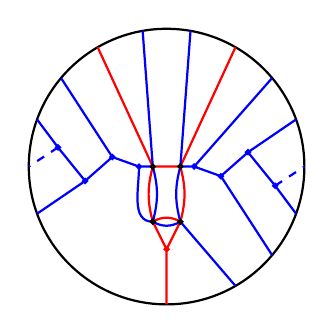
\begin{tikzpicture}[baseline=-.5ex,xscale=0.35,yscale=0.35]
\draw[thick] (0,0) circle (5cm);
\draw[blue, thick, fill] (-0.5,0) -- (-1,0) circle (2pt) (-1,0) -- (170:2) circle (2pt) -- (140:5) (170:2) -- (190:3) circle (2pt) -- (200:5) (190:3) -- (170:4) circle (2pt) -- (160:5);
\draw[blue, thick, dashed] (170:4) -- (180:5);
%
\draw[blue, thick, fill] (0.5,0) -- (1,0) circle (2pt) -- (40:5) (1,0) -- (-10:2) circle (2pt) -- (-40:5) (-10:2) -- (10:3) circle (2pt) -- (20:5) (10:3) -- (-10:4) circle (2pt) -- (-20:5);
\draw[blue, thick, dashed] (-10:4) -- (0:5);
%
\draw[blue, thick] (180:1) to[out=-90,in=-180] (-0.5,-2);
%
\draw[red, thick] (180:0.5) -- (120:5) (0:0.5) -- (60:5) (0:0.5) -- (180:0.5);
\draw[blue, thick] (180:0.5) -- (100:5) (0:0.5) -- (80:5);
%
\draw[red, thick] (-0.5,0) to[out=-105,in=105] (-0.5,-2) (0.5,0) to[out=-75,in=75] (0.5,-2) (-0.5,-2) to[out=30, in=150] (0.5,-2);
\draw[blue, thick] (-0.5,0) to[out=-75,in=75] (-0.5,-2) (0.5,0) to[out=-105,in=105] (0.5,-2) (-0.5,-2) to[out=-30, in=-150] (0.5,-2) -- (300:5);
\draw[red, thick, fill] (-0.5,-2) -- (0, -3) circle (2pt) (0,-3) -- (0.5, -2) (0,-3) -- (0,-5);
\draw[fill=white, thick] (-0.5,0) circle (2pt) (0.5,0) circle (2pt) (-0.5,-2) circle (2pt) (0.5,-2) circle (2pt);
\end{tikzpicture}\arrow[r,leftrightarrow,"\Move{II}^2"]&
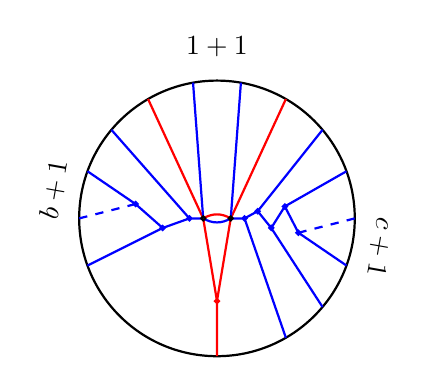
\begin{tikzpicture}[baseline=-.5ex,xscale=0.35,yscale=0.35]
\draw[thick] (0,0) circle (5cm);
\draw[blue, thick, fill] (-0.5,0) -- (-1,0) circle (2pt) -- (140:5) (-1,0) -- (190:2) circle (2pt) -- (200:5) (190:2) -- (170:3) circle (2pt) -- (160:5);
\draw[blue, thick, dashed] (170:3) -- (180:5);
%
\draw[blue, thick, fill] (0.5,0) -- (1,0) circle (2pt) -- (-60:5) (1,0) -- (10:1.5) circle (2pt) -- (40:5) (10:1.5) -- (-10:2) circle (2pt) -- (-40:5) (-10:2) -- (10:2.5) circle (2pt) -- (20:5) (10:2.5) -- (-10:3) circle (2pt) -- (-20:5);
\draw[blue, thick, dashed] (-10:3) -- (0:5);
%
\draw[red, thick] (-0.5,0) -- (120:5) (0.5,0) -- (60:5) (-0.5,0) to[out=30,in=150] (0.5,0);
\draw[blue, thick] (-0.5,0) -- (100:5) (0.5,0) -- (80:5) (-0.5,0) to[out=-30,in=-150] (0.5,0);
\draw[red, thick, fill] (-0.5,0) -- (0,-3) circle (2pt) -- (0.5,0) (0,-3) -- (0,-5);
\draw[fill=white, thick] (-0.5,0) circle (2pt) (0.5,0) circle (2pt);
%
\curlybrace[]{130}{210}{5.5};
\draw (170:6) node[rotate=80] {$b+1$};
\curlybrace[]{-70}{50}{5.5};
\draw (-10:6) node[rotate=-100] {$c+1$};
\curlybrace[]{70}{110}{5.5};
\draw (90:5.5) node[above] {$1+1$};
\end{tikzpicture}
\end{tikzcd}
\]
where the right one is equivalent to the $3$-graph $\ngraph(1,b,c)$ via the Move~\Move{II} as claimed.

\subsection{Equivalence between $\mathscr{G}^{\mathsf{brick}}(a,b,c)$ and $\mathscr{G}(a,b,c)$}\label{appendix:Ngraph of type abc}

\[
\begin{tikzcd}
\begin{tikzpicture}[baseline=-.5ex,scale=1]
\draw[thick, rounded corners] (-4,-1) rectangle (3,1);
\begin{scope}
\clip (-4,-1) rectangle (3,1);
%
\draw[color=cyclecolor1, line cap=round, line width=5, opacity=0.5] (-3.5,0.5) -- (-1, 0.5) (-2.5,-0.5) -- (-2,-0.5) (-0.5, 0.5) -- (0, 0.5) (1, -0.5) -- (1.5, -0.5) (2, -0.5) -- (2.5, -0.5);
\draw[color=cyclecolor2, line cap=round, line width=5, opacity=0.5] (-3,-0.5) -- (-2.5,-0.5) (-2, -0.5) -- (-1.5, -0.5) (-1, 0.5) -- (-0.5, 0.5) (0,0.5) -- (0.5,0.5) (1.5, -0.5) -- (2, -0.5);
\draw[color=cyan, line cap=round, line width=5, opacity=0.5] (-1, 0.5) -- (-1, -0.5)
(-1, -0.5) -- (1, -0.5)
(-0.5, 0.5) -- (-0.5, -0.5)
(0, 0.5) -- (0, -0.5)
(0.5, -0.5) -- (0.5, 0.5)
 (-1.5,-0.5) -- (-1,-0.5);
%
\draw[thick, blue] 
(-4,-0.5) -- (4, -0.5)
(-4, 0.5) -- (4, 0.5)
;
%
\draw[thick, blue, fill] 
(-3.5, -0.5) -- (-3.5, 0.5) circle (1pt)
(-3, -1) -- (-3, -0.5) circle (1pt)
(-2.5, -1) -- (-2.5, -0.5) circle (1pt)
(-2, -1) -- (-2, -0.5) circle (1pt)
(-1.5,-1) -- (-1.5,-0.5) circle (1pt)
(-1, -0.5) -- (-1, 0.5) circle (1pt)
(-0.5, -0.5) -- (-0.5, 0.5) circle (1pt)
(0, -0.5) -- (0, 0.5) circle (1pt)
(0.5, -0.5) -- (0.5, 0.5) circle (1pt)
(1, -1) -- (1, -0.5) circle (1pt)
(1.5, -1) -- (1.5, -0.5) circle (1pt)
(2, -1) -- (2, -0.5) circle (1pt)
(2.5, -1) -- (2.5,-0.5) circle (1pt);
%
\draw[thick, red] (-3.5,-1) -- (-3.5,-0.5) (-1, -1) -- (-1, -0.5) (-0.5,-1) -- (-0.5, -0.5) (0,-0.5) -- (0, -1) (0.5, -1) -- (0.5,-0.5);
\draw[thick, red, rounded corners] (-4,0) -- (-3.75,0) -- (-3.5,-0.5) (-3.5, -0.5) -- (-3.25, 0) -- (-1.25, 0) -- (-1, -0.5) 
(-1, -0.5) -- (-0.75, 0) -- (-0.5, -0.5) 
(-0.5, -0.5) -- (-0.25, 0) -- (0, -0.5)
(0, -0.5) -- (0.25,0) -- (0.5,-0.5)
(0.5, -0.5) -- (0.75, 0) -- (1, 0) -- (3,0);
\foreach \x in {-3.5, -1, -0.5, 0, 0.5} {
\draw[thick, fill=white] (\x,-0.5) circle (1pt) ;
}
\end{scope}
\draw (-2.25, -1) node[below] {$\underbrace{\hphantom{\hspace{1.8cm}}}_{a}$};
\draw (-.25, -1) node[below] {$\underbrace{\hphantom{\hspace{1.8cm}}}_{b-1}$};
\draw (1.75, -1) node[below] {$\underbrace{\hphantom{\hspace{1.8cm}}}_{c}$};
\end{tikzpicture}
\arrow[d, "\Move{I}^*\Move{II}^*"]\\
\begin{tikzpicture}[baseline=-.5ex,scale=1]
\draw[thick, rounded corners] (-4,-1.5) rectangle (3,1);
\begin{scope}
\clip (-4,-1.5) rectangle (3,1);
%
\draw[color=cyclecolor1, rounded corners, line cap=round, line width=5, opacity=0.5] (-3.5,0.5) -- (-1, 0.5) -- (-1, -1) (-2.5,-0.5) -- (-2,-0.5) (-0.5, -1) -- (0, -1) (1, -0.5) -- (1.5, -0.5) (2, -0.5) -- (2.5, -0.5);
\draw[color=cyclecolor2, line cap=round, line width=5, opacity=0.5] (-3,-0.5) -- (-2.5,-0.5) (-2, -0.5) -- (-1.5, -0.5) (-1, -1) -- (-0.5, -1) (0,-1) -- (0.5,-1) (1.5, -0.5) -- (2, -0.5);
\draw[color=cyan, rounded corners, line cap=round, line width=5, opacity=0.5] 
(0.5, -0.5) -- (1, -0.5)
(-1, -0.5) -- (-0.75, 0) -- (0.25, 0) -- (0.5, -0.5)
(-1.5,-0.5) -- (-1,-0.5);
%
\draw[thick, blue, rounded corners] 
(-4,-0.5) -- (4, -0.5)
(-4, 0.5) -- (-1, 0.5) -- (-1, -0.5)
(0.5, -0.5) -- (0.5, 0.5) -- (3,0.5)
;
%
\draw[thick, blue, fill] 
(-3.5, -0.5) -- (-3.5, 0.5) circle (1pt)
(-3, -1.5) -- (-3, -0.5) circle (1pt)
(-2.5, -1.5) -- (-2.5, -0.5) circle (1pt)
(-2, -1.5) -- (-2, -0.5) circle (1pt)
(-1.5,-1.5) -- (-1.5,-0.5) circle (1pt)
(1, -1.5) -- (1, -0.5) circle (1pt)
(1.5, -1.5) -- (1.5, -0.5) circle (1pt)
(2, -1.5) -- (2, -0.5) circle (1pt)
(2.5, -1.5) -- (2.5,-0.5) circle (1pt);
%
\draw[thick, red, fill] 
(-3.5,-1.5) -- (-3.5,-0.5) 
(-1, -1.5) -- (-1, -1) circle (1pt) -- (-1, -0.5)
(-0.5,-1.5) -- (-0.5, -1) circle (1pt) -- (-1, -1) (-0.5, -1) -- (0, -1)
(0, -1.5) -- (0,-1) circle (1pt)
(0.5, -1.5) -- (0.5,-1) circle (1pt) -- (0.5, -0.5) (0.5, -1) -- (0, -1);
\draw[thick, red, rounded corners] (-4,0) -- (-3.75,0) -- (-3.5,-0.5) (-3.5, -0.5) -- (-3.25, 0) -- (-1.25, 0) -- (-1, -0.5) 
(-1, -0.5) -- (-0.75, 0) -- (0.25, 0) -- (0.5, -0.5)
(0.5, -0.5) -- (0.75, 0) -- (1, 0) -- (3,0);
%
\foreach \x in {-3.5, -1, 0.5} {
\draw[thick, fill=white] (\x,-0.5) circle (1pt) ;
}
\end{scope}
\end{tikzpicture}
\arrow[d, "\Move{II}^*"]\\
\begin{tikzpicture}[baseline=-.5ex,scale=1]
\draw[thick, rounded corners] (-4.5,-1.5) rectangle (3,1);
\begin{scope}
\clip (-4.5,-1.5) rectangle (3,1);
%
\draw[color=cyclecolor1, rounded corners, line cap=round, line width=5, opacity=0.5] (-1.5, -1) -- (-1, -1) (-3,-0.5) -- (-2.5,-0.5) (-0.5, -1) -- (0, -1) (0.5, 0) -- (1, 0) (1.5, 0) -- (2, 0);
\draw[color=cyclecolor2, line cap=round, line width=5, opacity=0.5] (-3.5,-0.5) -- (-3,-0.5) (-2.5, -0.5) -- (-2, -0.5) (-1, -1) -- (-0.5, -1) (0,-1) -- (0.5,-1) (1, 0) -- (1.5, 0);
\draw[color=cyan, rounded corners, line cap=round, line width=5, opacity=0.5] 
(-1.5, -1) -- (-1, -0.5) -- (-0.75, 0) -- (0.5, 0)
(-2,-0.5) -- (-1.5,-0.5) to[out=30, in=150] (-1, -0.5);
%
\draw[thick, blue, rounded corners] 
(-4.5,-0.5) -- (4, -0.5)
(-4.5, 0.5) -- (-1, 0.5) -- (-1, -0.5)
(2.5, -0.5) -- (2.5, 0.5) -- (3,0.5)
(-4, -0.5) -- (-4, 0.25) -- (-1.5, 0.25) -- (-1.5, -0.5)
;
%
\draw[thick, blue, fill] 
(-3.5, -1.5) -- (-3.5, -0.5) circle (1pt)
(-3, -1.5) -- (-3, -0.5) circle (1pt)
(-2.5, -1.5) -- (-2.5, -0.5) circle (1pt)
(-2, -1.5) -- (-2, -0.5) circle (1pt)
;
\draw[thick, blue, rounded corners]
(1, -1.5) -- (1, -1) -- (0.5, -0.5)
(1.5, -1.5) -- (1.5, -1) -- (1, -0.5)
(2, -1.5) -- (2, -1) -- (1.5, -0.5)
(2.5, -1.5) -- (2.5, -1) -- (2,-0.5);
%
\draw[thick, red, fill] 
(-4,-1.5) -- (-4,-0.5) 
(-1.5, -0.5) -- (-1.5, -1) circle (1pt) -- (-1, -1)
(-1, -0.5) -- (-1.5, -1)
(-1, -1.5) -- (-1, -1) circle (1pt)
(-0.5,-1.5) -- (-0.5, -1) circle (1pt) -- (-1, -1) (-0.5, -1) -- (0, -1)
(0, -1.5) -- (0,-1) circle (1pt)
(0.5, -1.5) -- (0.5,-1) circle (1pt) -- (0.5, -0.5) (0.5, -1) -- (0, -1)
(0.5, -0.5) -- (0.5, 0) circle (1pt)
(1, -0.5) -- (1, 0) circle (1pt)
(1.5, -0.5) -- (1.5, 0) circle (1pt)
(2, -0.5) -- (2, 0) circle (1pt)
(2.5, -0.5) -- (2, 0)
;
\draw[thick, red, rounded corners] (-4.5,0) -- (-4.25,0) -- (-4,-0.5) (-4, -0.5) -- (-3.75, 0) -- (-1.75, 0) -- (-1.5, -0.5) 
(-1, -0.5) -- (-0.75, 0) -- (2, 0)
(2.5, -0.5) -- (2.75, 0) -- (3,0)
(0.5, -0.5) to[out=-30, in=-150] (1, -0.5)
(1, -0.5) to[out=-30, in=-150] (1.5, -0.5)
(1.5, -0.5) to[out=-30, in=-150] (2, -0.5)
(2, -0.5) to[out=-30, in=-150] (2.5, -0.5)
(-1.5, -0.5) to[out=30, in=150] (-1, -0.5)
;
%
\foreach \x in {-4, -1.5, -1, 0.5, 1, 1.5, 2, 2.5} {
\draw[thick, fill=white] (\x,-0.5) circle (1pt) ;
}
\end{scope}
\end{tikzpicture}
\arrow[d, "\Move{II}^*"]\\
\begin{tikzpicture}[baseline=-.5ex,scale=1]
\draw[thick, rounded corners, fill=black!10] (-4.5,-1.5) rectangle (3,1);
\fill[white, rounded corners] (-3.25, 0.25) -- (2.25, 0.25) -- (2.25, -0.25) -- (-0.75, -0.25) -- (-0.75, -0.75) -- (0.5, -0.75) -- (0.75, -1) -- (0.75, -1.25) -- (-1.75, -1.25) -- (-1.75, -1) -- (-1.25, -0.5) -- (-1.5, -0.25) -- (-3.25, -0.25) -- cycle;
\begin{scope}
\clip (-4.5,-1.5) rectangle (3,1);
%
\draw[color=cyclecolor1, rounded corners, line cap=round, line width=5, opacity=0.5] (-1.5, -1) -- (-1, -1) (-2.5,0) -- (-2,0) (-0.5, -1) -- (0, -1) (0.5, 0) -- (1, 0) (1.5, 0) -- (2, 0);
\draw[color=cyclecolor2, line cap=round, line width=5, opacity=0.5] (-3,0) -- (-2.5,0) (-2, 0) -- (-1.5, 0) (-1, -1) -- (-0.5, -1) (0,-1) -- (0.5,-1) (1, 0) -- (1.5, 0);
\draw[color=cyan, rounded corners, line cap=round, line width=5, opacity=0.5] 
(-1.5, -1) -- (-1, -0.5) -- (-0.75, 0) -- (0.5, 0)
(-1.5,0) -- (-1, -0.5);
%
\draw[thick, blue, rounded corners] 
(-4.5,-0.5) -- (4, -0.5)
(-4.5, 0.5) -- (-1, 0.5) -- (-1, -0.5)
(2.5, -0.5) -- (2.5, 0.5) -- (3,0.5)
(-4, -0.5) -- (-4, 0.25) -- (-3.5, 0.25) -- (-3.5, -0.5)
;
%
\draw[thick, blue, rounded corners] 
(-3.5, -1.5) -- (-3.5, -1) -- (-3, -0.5)
(-3, -1.5) -- (-3, -1) -- (-2.5, -0.5)
(-2.5, -1.5) -- (-2.5, -1) -- (-2, -0.5)
(-2, -1.5) -- (-2, -1) -- (-1.5, -0.5)
(1, -1.5) -- (1, -1) -- (0.5, -0.5)
(1.5, -1.5) -- (1.5, -1) -- (1, -0.5)
(2, -1.5) -- (2, -1) -- (1.5, -0.5)
(2.5, -1.5) -- (2.5, -1) -- (2,-0.5);
%
\draw[thick, red, fill] 
(-4,-1.5) -- (-4,-0.5) 
(-1.5, -0.5) -- (-1.5, -1) circle (1pt) -- (-1, -1)
(-1, -0.5) -- (-1.5, -1)
(-1, -1.5) -- (-1, -1) circle (1pt)
(-0.5,-1.5) -- (-0.5, -1) circle (1pt) -- (-1, -1) (-0.5, -1) -- (0, -1)
(0, -1.5) -- (0,-1) circle (1pt)
(0.5, -1.5) -- (0.5,-1) circle (1pt) -- (0.5, -0.5) (0.5, -1) -- (0, -1)
(0.5, -0.5) -- (0.5, 0) circle (1pt)
(1, -0.5) -- (1, 0) circle (1pt)
(1.5, -0.5) -- (1.5, 0) circle (1pt)
(2, -0.5) -- (2, 0) circle (1pt)
(2.5, -0.5) -- (2, 0)
(-3.5, -0.5) -- (-3, 0) (-3, 0) -- (-1.5,0)
(-3, -0.5) -- (-3, 0) circle (1pt)
(-2.5, -0.5) -- (-2.5, 0) circle (1pt)
(-2, -0.5) -- (-2, 0) circle (1pt)
(-1.5, -0.5) -- (-1.5, 0) circle (1pt)
;
\draw[thick, red, rounded corners] (-4.5,0) -- (-4.25,0) -- (-4,-0.5) (-4, -0.5) -- (-3.75, 0) -- (-3.5, -0.5) 
(-1, -0.5) -- (-0.75, 0) -- (2, 0)
(2.5, -0.5) -- (2.75, 0) -- (3,0)
(0.5, -0.5) to[out=-30, in=-150] (1, -0.5)
(1, -0.5) to[out=-30, in=-150] (1.5, -0.5)
(1.5, -0.5) to[out=-30, in=-150] (2, -0.5)
(2, -0.5) to[out=-30, in=-150] (2.5, -0.5)
(-1.5, 0) -- (-1, -0.5)
(-3.5, -0.5) to[out=-30, in=-150] (-3, -0.5)
(-3, -0.5) to[out=-30, in=-150] (-2.5, -0.5)
(-2.5, -0.5) to[out=-30, in=-150] (-2, -0.5)
(-2, -0.5) to[out=-30, in=-150] (-1.5, -0.5)
;
%
\foreach \x in {-4, -3.5, -3, -2.5, -2, -1.5, -1, 0.5, 1, 1.5, 2, 2.5} {
\draw[thick, fill=white] (\x,-0.5) circle (1pt) ;
}
\end{scope}
\end{tikzpicture}
\end{tikzcd}
\]

The innermost $N$-graph is the same as $\overline{\ngraph(a,b,c)}$ up to Legendrian mutations, which is $\boundary$-Legendrian isotopic to the Legendrian Coxeter mutation of $\ngraph(a,b,c)$ by Proposition~\ref{proposition:effect of Legendrian Coxeter mutation}.


%\subsection{Equivalence between $\tilde{\mathscr{G}}(a,b,b)$ and a stabilization of $\mathscr{G}(a,b,b)$}\label{appendix:Ngraph of type abb}

\subsection{Equivalence between $\mathscr{G}^{\mathsf{brick}}(\exdynD_n)$ and $\mathscr{G}(\exdynD_n)$}\label{appendix:Ngraph of type affine Dn}

We first show that $\ngraph^{\mathsf{brick}}(\exdynD_n)$ is Legendrian mutation equivalent to the following $N$-graph up to $\boundary$-Legendrian isotopy:
\[
\begin{tikzcd}
\ngraph(\exdynD_n)'\coloneqq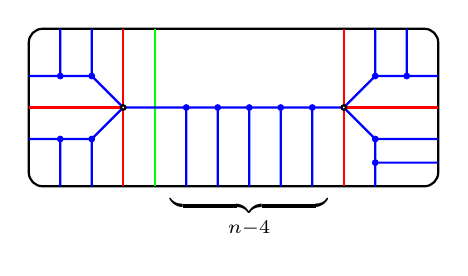
\begin{tikzpicture}[baseline=-.5ex,scale=0.4]
\draw[rounded corners=5, thick] (-6.5, -2.5) rectangle (6.5, 2.5);
\draw (0.5, -2.5) node[below] {$\underbrace{\hphantom{\hspace{2cm}}}_{n-4}$};
\clip[rounded corners=5] (-6.5, -2.5) rectangle (6.5, 2.5);
\draw[thick, blue, fill]
%(-2.5, -2.5) -- (-2.5,0) circle (2pt)
(-0.5, -2.5) -- (-0.5,0) circle (2pt)
(1.5, -2.5) -- (1.5,0) circle (2pt)
;
\begin{scope}[xscale=-1]
\draw[thick, blue, fill]
(-2.5, -2.5) -- (-2.5,0) circle (2pt)
(-0.5, -2.5) -- (-0.5,0) circle (2pt)
(1.5, -2.5) -- (1.5,0) circle (2pt)
;
\end{scope}
\draw[thick, green, rounded corners] (-2.5, 2.5) -- (-2.5, -2.5);
\draw[thick, red] 
(-3.5, -2.5) -- (-3.5, 2.5)
(-6.5, 0) -- (-3.5, 0)
;
\draw[thick, red] 
(3.5, 2.5) -- (3.5, -2.5)
(6.5, 0) -- (3.5, 0)
;
\draw[thick, blue, fill] 
%
(-3.5, 0) -- (3.5, 0)
(-3.5, 0) -- (-4.5, 1) circle (2pt) -- (-4.5, 2.5)
(-4.5, 1) -- (-6.5, 1)
(-5.5, 1) circle (2pt) -- (-5.5, 2.5)
%
(-3.5, 0) -- (-4.5, -1) circle (2pt) -- (-4.5, -2.5)
(-4.5, -1) -- (-6.5, -1)
(-5.5, -1) circle (2pt) -- (-5.5, -3)
;
\begin{scope}[xscale=-1]
\draw[thick, blue, fill] 
%
(-3.5, 0) -- (-4.5, 1) circle (2pt) -- (-4.5, 2.5)
(-4.5, 1) -- (-6.5, 1)
(-5.5, 1) circle (2pt) -- (-5.5, 2.5)
%
(-3.5, 0) -- (-4.5, -1) circle (2pt) -- (-4.5, -2.5)
(-4.5, -1) -- (-6.5, -1)
(-4.5, -1.75) circle (2pt) -- (-6.5, -1.75)
;
\end{scope}
\draw[thick, fill=white] (-3.5, 0) circle (2pt) (3.5, 0) circle (2pt);
\end{tikzpicture}
\arrow[r, "\boundary\text{-Leg. iso.}"'] & 
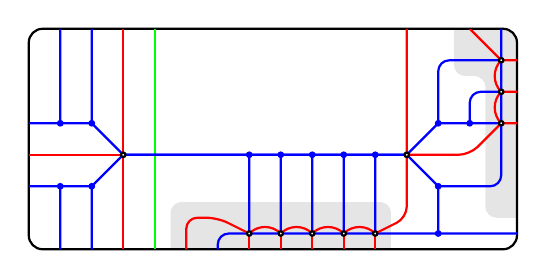
\begin{tikzpicture}[baseline=-.5ex,scale=0.4]
\draw[rounded corners=5, thick] (-7.5, -3) rectangle (8, 4);
\clip[rounded corners=5] (-7.5, -3) rectangle (8, 4);
\fill[opacity=0.1, rounded corners] (-3, -4) -- (-3, -1.5) -- (4, -1.5) -- (4, -4) -- cycle;
\fill[opacity=0.1, rounded corners] (7, -2) -- (9,-2) -- (9, 5) -- (6, 5) -- (6, 2.5) -- (7, 2.5) -- cycle;
\draw[thick, red]
(-0.5, -2.5) -- (-0.5, -3)
(0.5, -2.5) -- (0.5, -3)
(1.5, -2.5) -- (1.5, -3)
(2.5, -2.5) -- (2.5, -3)
(3.5, -2.5) -- (3.5, -3)
;
\draw[thick, blue, fill]
(-0.5, -2.5) -- (-0.5,0) circle (2pt)
(0.5, -2.5) -- (0.5,0) circle (2pt)
(1.5, -2.5) -- (1.5,0) circle (2pt)
(2.5, -2.5) -- (2.5, 0) circle (2pt)
(3.5, -2.5) -- (3.5, 0) circle (2pt)
;
\draw[thick, blue, rounded corners]
(-0.5, -2.5) -- (-1.5, -2.5) -- (-1.5, -3)
(-0.5, -2.5) -- (3.5, -2.5) -- (8, -2.5)
;
\draw[thick, green, rounded corners] (-3.5, 4) -- (-3.5, -3);
\draw[thick, red] 
(-4.5, -3) -- (-4.5, 4)
(-7.5, 0) -- (-4.5, 0)
;
\draw[thick, red, rounded corners] 
(4.5, 4) -- (4.5, -2) -- (3.5, -2.5)
(-0.5, -2.5) to[out=45,in=135] (0.5, -2.5)
(0.5, -2.5) to[out=45,in=135] (1.5, -2.5)
(1.5, -2.5) to[out=45,in=135] (2.5, -2.5)
(2.5, -2.5) to[out=45,in=135] (3.5, -2.5)
(-0.5, -2.5) -- (-1.5, -2) -- (-2.5, -2) -- (-2.5, -3)
(4.5, 0) -- (6.5, 0) -- (7.5, 1)
(7.5,1) to[out=135, in=-135] (7.5,2)
(7.5,2) to[out=135, in=-135] (7.5,3)
(7.5,3) -- (6.5, 4)
(7.5,1) -- (8, 1)
(7.5,2) -- (8, 2)
(7.5,3) -- (8, 3)
;
\draw[thick, blue, fill] 
%
(-4.5, 0) -- (4.5, 0)
(-4.5, 0) -- (-5.5, 1) circle (2pt) -- (-5.5, 4)
(-5.5, 1) -- (-7.5, 1)
(-6.5, 1) circle (2pt) -- (-6.5, 4)
%
(-4.5, 0) -- (-5.5, -1) circle (2pt) -- (-5.5, -3)
(-5.5, -1) -- (-7.5, -1)
(-6.5, -1) circle (2pt) -- (-6.5, -3)
;
\draw[thick, blue, rounded corners]
(5.5, -1) -- (7.5, -1) -- (7.5, 4)
(5.5, 1) -- (5.5, 3) -- (7.5, 3)
(5.5, 1) -- (7.5, 1)
(6.5, 1) circle (2pt) -- (6.5, 2) -- (7.5, 2)
(5.5, -2.5) circle (2pt) -- (5.5, -1)
;
\begin{scope}[rotate=180]
\draw[thick, blue, fill] 
%
(-4.5, 0) -- (4.5, 0)
(-4.5, 0) -- (-5.5, 1) circle (2pt)
%
(-4.5, 0) -- (-5.5, -1) circle (2pt)
;
\end{scope}
\draw[thick, fill=white] 
(-4.5, 0) circle (2pt) (4.5, 0) circle (2pt)
(7.5, 1) circle (2pt) (7.5, 2) circle (2pt) (7.5, 3) circle (2pt)
(-0.5, -2.5) circle (2pt) (0.5, -2.5) circle (2pt) (1.5, -2.5) circle (2pt) (2.5, -2.5) circle (2pt) (3.5, -2.5) circle (2pt)
;
\end{tikzpicture}
\arrow[ld, sloped, "\Move{I}^*","\Move{II}^*"']\\
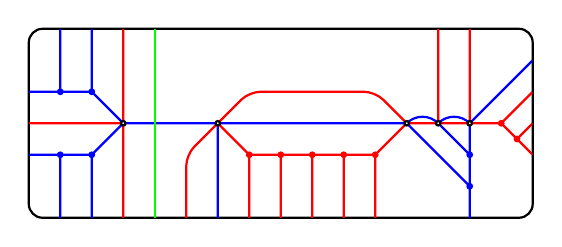
\begin{tikzpicture}[baseline=-.5ex,scale=0.4]
\draw[rounded corners=5, thick] (-7.5, -3) rectangle (8.5, 3);
\clip[rounded corners=5] (-7.5, -3) rectangle (8.5, 3);
\draw[thick, red, fill]
(-1.5, 0) -- (-0.5, -1) circle (2pt) -- (-0.5, -3)
(0.5, -1) circle (2pt) -- (0.5, -3)
(1.5, -1) circle (2pt) -- (1.5, -3)
(2.5, -1) circle (2pt) -- (2.5, -3)
(6.5, 0) -- (4.5,0)
(4.5, 0) -- (3.5, -1) circle (2pt) -- (3.5, -3)
(-0.5, -1) -- (3.5, -1)
(6.5, 0) -- (6.5, 3)
(6.5, 0) -- (7.5, 0) circle (2pt) -- +(1,1)
+(0,0) -- ++(0.5, -0.5) circle (2pt) -- +(0.5, 0.5)
+(0,0) -- +(0.5, -0.5)
;
\draw[thick, red, rounded corners]
(-1.5, 0) -- (-2.5, -1) -- (-2.5, -3)
(-4.5, 3) -- (-4.5, -3)
(-4.5, 0) -- (-7.5, 0)
(-1.5, 0) -- (-0.5, 1) -- (3.5, 1) -- (4.5, 0)
(5.5, 3) -- (5.5, 0)
;
\draw[thick, blue, fill] 
%
(-4.5, 0) -- (-5.5, 1) circle (2pt) -- (-5.5, 3.5)
(-5.5, 1) -- (-7.5, 1)
(-6.5, 1) circle (2pt) -- (-6.5, 3.5)
%
(-4.5, 0) -- (-5.5, -1) circle (2pt) -- (-5.5, -3)
(-5.5, -1) -- (-7.5, -1)
(-6.5, -1) circle (2pt) -- (-6.5, -3)
%
(4.5, 0) -- (6.5, -2) circle (2pt)
(6.5, -1) circle (2pt) -- (5.5, 0)
(6.5, -1) -- (6.5, -3)
(6.5, -1) -- (6.5, 0)
;
\draw[thick, blue, rounded corners]
(-4.5, 0) -- (-2.5, 0) -- (-1.5, 0)
(-1.5, 0) -- (-1.5, -3)
(-1.5, 0) -- (-0.5, 0) -- (3.5, 0) -- (4.5, 0)
(4.5, 0) to[out=45, in=135] (5.5, 0)
(5.5, 0) to[out=45, in=135] (6.5, 0) 
(6.5, 0) -- (8.5, 2)
;
\draw[thick, green] 
(-3.5, 3) -- (-3.5, -3)
;
\draw[thick, fill=white] 
(-4.5, 0) circle (2pt) (-1.5, 0) circle (2pt) (4.5, 0) circle (2pt) (5.5, 0) circle (2pt) (6.5, 0) circle (2pt)
;
\end{tikzpicture}
\arrow[r,sloped, "\Move{II}^2"',"\boundary\text{-Leg. iso.}"] &
%\begin{tikzpicture}[baseline=-.5ex,scale=0.6]
%\draw[rounded corners=5, thick] (-7.5, -3) rectangle (6.5, 3);
%\clip[rounded corners=5] (-7.5, -3) rectangle (6.5, 3);
%\draw[thick, red, fill]
%(-1.5, 0) -- (-0.5, 0) circle (2pt) -- (-0.5, -3)
%(0.5, 0) circle (2pt) -- (0.5, -3)
%(1.5, 0) circle (2pt) -- (1.5, -3)
%(2.5, 0) circle (2pt) -- (2.5, -3)
%(4.5, 0) -- (3.5, 0) circle (2pt) -- (3.5, -3)
%(-0.5, 0) -- (3.5, 0)
%(-1.5, 2) -- (-1.5, 3)
%(4.5, 0) -- (5.5, 0) circle (2pt) -- +(1,-1)
%+(0,0) -- ++(0.5, 0.5) circle (2pt) -- +(0.5, 0.5)
%+(0,0) -- +(0.5, -0.5)
%(-1.5, 0) -- (-2.5, 1) circle (2pt) -- (-2.5, 3)
%;
%\draw[thick, red, rounded corners]
%(-2.5, 1) -- (-1.5, 2) circle (2pt) -- (4.5, 2) -- (4.5, 0)
%(-1.5, 0) -- (-2.5, -1) -- (-2.5, -3)
%(-4.5, 3) -- (-4.5, -3)
%(-4.5, 0) -- (-7.5, 0)
%;
%\draw[thick, blue, fill] 
%%
%(-4.5, 0) -- (-5.5, 1) circle (2pt) -- (-5.5, 3.5)
%(-5.5, 1) -- (-7.5, 1)
%(-6.5, 1) circle (2pt) -- (-6.5, 3.5)
%%
%(-4.5, 0) -- (-5.5, -1) circle (2pt) -- (-5.5, -3)
%(-5.5, -1) -- (-7.5, -1)
%(-5.5, -1.75) circle (2pt) -- (-7.5, -1.75)
%;
%\draw[thick, blue, rounded corners]
%(-4.5, 0) -- (-2.5, 0) -- (-1.5, 0)
%(-1.5, 0) -- (-1.5, -3)
%(-1.5, 0) -- (-0.5, 1) -- (3.5, 1) -- (4.5, 0)
%(4.5, 0) -- (4.5, -3)
%(4.5, 0) -- ++(3,3)
%;
%\draw[thick, green] 
%(-3.5, 3) -- (-3.5, -3)
%;
%\end{tikzpicture}
%\arrow[d,"\boundary\text{-Leg. Iso.}"]\\
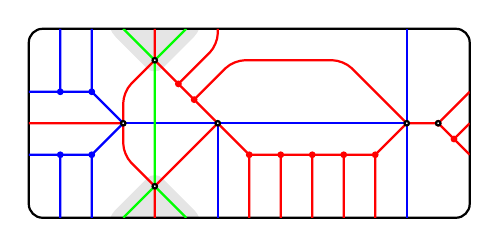
\begin{tikzpicture}[baseline=-.5ex,scale=0.4]
\draw[rounded corners=5, thick] (-7.5, -3) rectangle (6.5, 3);
\clip[rounded corners=5] (-7.5, -3) rectangle (6.5, 3);
\fill[opacity=0.1, rounded corners] (-5, 4) -- (-5, 3) -- (-3.5, 1.5) -- (-2, 3) -- (-2, 4) -- cycle;
\fill[opacity=0.1, rounded corners] (-5, -4) -- (-5, -3) -- (-3.5, -1.5) -- (-2, -3) -- (-2, -4) -- cycle;
\draw[thick, red, fill]
(-1.5, 0) -- (-0.5, -1) circle (2pt) -- (-0.5, -3)
(0.5, -1) circle (2pt) -- (0.5, -3)
(1.5, -1) circle (2pt) -- (1.5, -3)
(2.5, -1) circle (2pt) -- (2.5, -3)
(4.5, 0) -- (3.5, -1) circle (2pt) -- (3.5, -3)
(-0.5, -1) -- (3.5, -1)
(4.5, 0) -- (5.5, 0) circle (2pt) -- +(1,1)
+(0,0) -- ++(0.5, -0.5) circle (2pt) -- +(0.5, 0.5)
+(0,0) -- +(0.5, -0.5)
(-1.5, 0) -- (-2.25, 0.75) circle (2pt) -- (-2.75, 1.25) circle (2pt) -- (-3.5, 2)
(-3.5, 2) -- (-3.5, 3)
(-1.5, 0) -- (-2.5, -1) -- (-3.5, -2) 
(-3.5, -2) -- (-3.5, -3)
;
\draw[thick, red, rounded corners]
(-2.25, 0.75) -- (-1, 2) -- (2.5, 2) -- (4.5, 0)
(-2.75,1.25) -- (-1.5, 2.5) -- (-1.5, 3)
(-3.5, 2) -- (-4.5, 1) -- (-4.5, -1) -- (-3.5, -2)
(-4.5, 0) -- (-7.5, 0)
;
\draw[thick, blue, fill] 
%
(-4.5, 0) -- (-5.5, 1) circle (2pt) -- (-5.5, 3.5)
(-5.5, 1) -- (-7.5, 1)
(-6.5, 1) circle (2pt) -- (-6.5, 3.5)
%
(-4.5, 0) -- (-5.5, -1) circle (2pt) -- (-5.5, -3)
(-5.5, -1) -- (-7.5, -1)
(-6.5, -1) circle (2pt) -- (-6.5, -3)
;
\draw[thick, blue, rounded corners]
(-4.5, 0) -- (-2.5, 0) -- (-1.5, 0)
(-1.5, 0) -- (-1.5, -3)
(-1.5, 0) -- (-0.5, 0) -- (3.5, 0) -- (4.5, 0)
(4.5, 0) -- (4.5, -3)
(4.5, 0) -- ++(0,3)
;
\draw[thick, green] 
(-3.5, 2) -- (-3.5, -2)
(-4.5, 3) -- (-3.5, 2) -- (-2.5, 3)
(-4.5, -3) -- (-3.5, -2) -- (-2.5, -3)
;
\draw[thick, fill=white] 
(-4.5, 0) circle (2pt)
(-3.5, 2) circle (2pt) (-3.5, -2) circle (2pt)
(-1.5, 0) circle (2pt) (4.5, 0) circle (2pt) (5.5, 0) circle (2pt) (6.5, 0)
;
\end{tikzpicture}
\arrow[ld, sloped, "\Move{II}^2"]\\
\begin{tikzpicture}[baseline=-.5ex,scale=0.4]
\draw[rounded corners=5, thick] (-7.5, -3) rectangle (6.5, 4);
\clip[rounded corners=5] (-7.5, -3) rectangle (6.5, 4);
\fill[opacity=0.1, rounded corners] (-0.5, 1.5) -- (-0.5, 5) -- (3, 5) -- (3, 1.5) -- cycle;
\draw[thick, red, fill]
(-1.5, 0) -- (-0.5, -1) circle (2pt) -- (-0.5, -3)
(0.5, -1) circle (2pt) -- (0.5, -3)
(1.5, -1) circle (2pt) -- (1.5, -3)
(2.5, -1) circle (2pt) -- (2.5, -3)
(4.5, 0) -- (3.5, -1) circle (2pt) -- (3.5, -3)
(-0.5, -1) -- (3.5, -1)
(4.5, 0) -- (5.5, 0) circle (2pt) -- +(1,1)
+(0,0) -- ++(0.5, -0.5) circle (2pt) -- +(0.5, 0.5)
+(0,0) -- +(0.5, -0.5)
(-1.5, 0) -- (-2.5, 1) -- (-3.5, 2)
(-1.5, 0) -- (-2.5, -1) -- (-3.5, -2) 
(-3.5, -2) -- (-3.5, -3)
;
\draw[thick, red, rounded corners]
(-1.5, 2) -- (-1.5, 1) -- (3.5, 1) -- (4.5, 0)
(-3.5, 2) -- (-4.5, 1) -- (-4.5, -1) -- (-3.5, -2)
(-4.5, 0) -- (-7.5, 0)
(-3.5, 2) -- (-1.5, 2)
(-1.5, 2) -- (0.5, 2)
(0.5, 2) -- (0.5, 4)
(0.5, 2) -- (2.5, 2) -- (2.5, 4)
;
\draw[thick, blue, fill] 
%
(-4.5, 0) -- (-5.5, 1) circle (2pt) -- (-5.5, 4)
(-5.5, 1) -- (-7.5, 1)
(-6.5, 1) circle (2pt) -- (-6.5, 4)
%
(-4.5, 0) -- (-5.5, -1) circle (2pt) -- (-5.5, -3)
(-5.5, -1) -- (-7.5, -1)
(-6.5, -1) circle (2pt) -- (-6.5, -3)
;
\draw[thick, blue, rounded corners]
(-4.5, 0) -- (-2.5, 0) -- (-1.5, 0)
(-1.5, 0) -- (-1.5, -3)
(-1.5, 0) -- (-0.5, 0) -- (3.5, 0) -- (4.5, 0)
(4.5, 0) -- (4.5, -3)
(4.5, 0) -- (4.5,4)
;
\draw[thick, green] 
(-3.5, 2) -- (-3.5, -2)
(-3.5, 4) -- (-3.5, 3) -- (-3.5, 2) to[out=-30,in=-150] (-1.5, 2) to[out=-30, in=-150] (0.5, 2)
(-4.5, -3) -- (-3.5, -2) -- (-2.5, -3)
;
\draw[thick, green, fill]
(-3.5, 3.5) circle (2pt)
(-3.5, 2.5) circle (2pt)
;
\draw[thick, green, rounded corners]
(0.5, 2) -- (-1.5, 3.5) -- (-3.5, 3.5)
(-1.5, 2) -- (-1.5, 2.5) -- (-3.5, 2.5)
(0.5, 2) -- (1.5, 3) -- (1.5, 4)
;
\draw[thick, fill=white] 
(-4.5, 0) circle (2pt) (-1.5, 0) circle (2pt) (4.5, 0) circle (2pt)
(-3.5, 2) circle (2pt) (-1.5, 2) circle (2pt) (0.5, 2) circle (2pt)
(-3.5, -2) circle (2pt)
;
\end{tikzpicture}
\arrow[r,sloped, "\Move{IV}"',"\boundary\text{-Leg. iso.}"]&
\begin{tikzpicture}[baseline=-.5ex,scale=0.4]
\draw[rounded corners=5, thick] (-7.5, -3) rectangle (6.5, 4);
\clip[rounded corners=5] (-7.5, -3) rectangle (6.5, 4);
\draw[thick, red, fill]
(-0.5, 0) circle (2pt) -- (-0.5, -3)
(0.5, 0) circle (2pt) -- (0.5, -3)
(1.5, 0) circle (2pt) -- (1.5, -3)
(2.5, 0) circle (2pt) -- (2.5, -3)
(4.5, 1) -- (3.5, 0) circle (2pt) -- (3.5, -3)
(-0.5, 0) -- (3.5, 0)
(4.5, 1) -- (5.5, 1) circle (2pt) -- +(1,1)
+(0,0) -- ++(0.5, -0.5) circle (2pt) -- +(0.5, 0.5)
+(0,0) -- +(0.5, -0.5)
(-2.5, 0) -- (-3.5, 1)
(-2.5, 0) -- (-3.5, -1) 
(-3.5, -1) -- (-3.5, -3)
;
\draw[thick, red, rounded corners]
(-2.5, 0) -- (-1.5, 0) -- (-0.5, 0)
(-2.5, 2) -- (-1.5, 2) -- (-0.5, 2) -- (3.5, 2) -- (4.5, 1)
(-3.5, 1) -- (-4.5, 0)
(-4.5, 0) -- (-3.5, -1)
(-4.5, 0) -- (-7.5, 0)
(-3.5, 1) -- (-3.5, 2) -- (-2.5, 2)
(-2.5, 2) -- (-2.5, 3) -- (-2.5, 4)
;
\draw[thick, blue, fill] 
%
(-3.5, 1) -- (-5.5, 1) circle (2pt) -- (-5.5, 4)
(-5.5, 1) -- (-7.5, 1)
(-6.5, 1) circle (2pt) -- (-6.5, 4)
%
(-3.5, -1) -- (-5.5, -1) circle (2pt) -- (-5.5, -3)
(-5.5, -1) -- (-7.5, -1)
(-6.5, -1) circle (2pt) -- (-6.5, -3)
;
\draw[thick, blue, rounded corners]
(-3.5, -1) -- (-3.5, 1)
(-1.5, -3) -- (-1.5, -2) -- (-2.5, -1) -- (-3.5, -1)
(-3.5, 1) -- (-1.5, 1) -- (-0.5, 1) -- (3.5, 1) -- (4.5, 1)
(4.5, 0) -- (4.5, -3)
(4.5, 0) -- (4.5,4)
;
\draw[thick, green] 
(-4.5, 0) -- (-2.5, 0)
(-4.5, 4) -- (-4.5, 0) 
(-4.5, -3) -- (-4.5, 0)
(-2.5, -3) -- (-2.5, 0)
;
\draw[thick, green, fill]
(-4.5, 3.5) circle (2pt)
(-4.5, 2.5) circle (2pt)
;
\draw[thick, green, rounded corners]
(-3.5, 4) -- (-3.5, 3.5) -- (-4.5, 3.5)
(-2.5, 2) -- (-3, 2.5) -- (-4.5, 2.5)
(-2.5, 0) -- (-2.5, 1) -- (-2.5, 2)
(-2.5, 2) -- (-1.5, 3) -- (-1.5, 4)
;
\draw[thick, fill=white] 
(-4.5, 0) circle (2pt) (-2.5, 0) circle (2pt) (4.5, 1) circle (2pt)
(-3.5, 1) circle (2pt) (-3.5, -1) circle (2pt) (-2.5, 2) circle (2pt)
;
\end{tikzpicture}
\arrow[ld, sloped, "\Move{II}^*"] \\
\begin{tikzpicture}[baseline=-.5ex,scale=0.4]
\draw[rounded corners=5, thick] (-7.5, -4) rectangle (7.5, 4);
\clip[rounded corners=5] (-7.5, -4) rectangle (7.5, 4);
\fill[opacity=0.1, rounded corners] (-8, 0.5) -- (-3, 0.5) -- (-3, -2.5) -- (8,-2.5) -- (8, -5) -- (-8, -5) --cycle;
;
\draw[thick, red, fill]
(0.5, 0) circle (2pt) -- (0.5, -4)
(1.5, 0) circle (2pt) -- (1.5, -4)
(2.5, 0) circle (2pt) -- (2.5, -4)
(3.5, 0) circle (2pt) -- (3.5, -4)
(5.5, 1) -- (4.5, 0) circle (2pt) -- (4.5, -4)
(0.5, 0) -- (4.5, 0)
(5.5, 1) -- (6.5, 1) circle (2pt) -- +(1,1)
+(0,0) -- ++(0.5, -0.5) circle (2pt) -- +(0.5, 0.5)
+(0,0) -- +(0.5, -0.5)
(-1.5, 0) -- (-3.5, 1)
(-1.5, 0) -- (-2.5, -1) 
(-3.5, -3) -- (-3.5, -4)
(-3.5, -1) -- (-2.5, -1) circle (2pt)
(-3.5, -2) -- (-2.5, -1)
(-2, -0.5) circle (2pt)
;
\draw[thick, red, rounded corners]
(-1.5, 0) -- (0.5, 0)
(-2.5, 2) -- (-1.5, 2) -- (-0.5, 2) -- (4.5, 2) -- (5.5, 1)
(-3.5, 1) -- (-4.5, 0)
(-4.5, 0) -- (-3.5, -1)
(-4.5, 0) -- (-7.5, 0)
(-3.5, 1) -- (-3.5, 2) -- (-2.5, 2)
(-1.5, 2) -- (-1.5, 4)
(-3.5, -3) to[out=135, in=-135] (-3.5, -2)
(-3.5, -2) to[out=135, in=-135] (-3.5, -1)
(-3.5, -3) -- (-2, -1.5) -- (-2, -0.5)
;
\draw[thick, blue, fill] 
%
(-3.5, 1) -- (-5.5, 1) circle (2pt) -- (-5.5, 4)
(-5.5, 1) -- (-7.5, 1)
(-6.5, 1) circle (2pt) -- (-6.5, 4)
%
(-3.5, -1) -- (-7.5, -1)
(-3.5, -1) -- (-3.5, -3)
;
\draw[thick, blue, rounded corners]
(-5.5, -4) -- (-5.5, -3) -- (-3.5, -3)
(-3.5, -1) -- (-3.5, 1)
(-0.5, -4) -- (-0.5, -3) -- (-2.5, -3) -- (-3.5, -3)
(-3.5, 1) -- (-1.5, 1) -- (-0.5, 1) -- (3.5, 1) -- (5.5, 1)
(5.5, 0) -- (5.5, -4)
(5.5, 0) -- (5.5,4)
(-3.5, -2) -- (-6.5, -2) -- (-6.5, -4)
;
\draw[thick, green] 
(-4.5, 0) -- (-1.5, 0)
(-4.5, 4) -- (-4.5, 0) 
(-4.5, -4) -- (-4.5, 0)
(-1.5, -4) -- (-1.5, 0)
(-1.5, 0) -- (-1.5, 2)
;
\draw[thick, green, fill]
(-4.5, 3.5) circle (2pt)
(-4.5, 2.5) circle (2pt)
;
\draw[thick, green, rounded corners]
(-2.5, 4) -- (-2.5, 3.5) -- (-4.5, 3.5)
(-1.5, 2) -- (-2, 2.5) -- (-4.5, 2.5)
(-1.5, 2) -- (-0.5, 3) -- (-0.5, 4)
;
\end{tikzpicture}
\arrow[r, "\boundary\text{-Leg. iso.}"] &
%(\ngraph^{\mathsf{brick}}(\exdynD_n),\nbasis^{\mathsf{brick}}(\exdynD_n))=
\begin{tikzpicture}[baseline=10ex, xscale=0.4, yscale=0.4]
\draw[rounded corners=5, thick] (0, 0) rectangle (14, 7);
\clip[rounded corners=5] (0, 0) rectangle (14, 7);
\fill[opacity=0.1, rounded corners] (-1, -1) rectangle (1.5, 4.5)
(12.5, 4.5) rectangle (14.5, -1);
\draw[blue,thick,rounded corners]
(0,3)--(6,3)--(8,2)--(9,2)--(10,1) (10,1)--(11,2)--(12,2)--(13,1) (13,1)--(13.5,2)--(14,2)
(0,5)--(6,5)--(8,6)--(14,6)
(1,3)--(1,5) (4,3)--(4,5) (10,0)--(10,1) (13,0)--(13,1);
\draw[red,thick,rounded corners] (0,1)--(6.5,1) (7.5,1)--(14,1)
(0,4)--(0.5,4)--(1,3) (1,3)--(2,4)--(3,4)--(4,3) (4,3)--(5,4)--(9,4)--(10,3) (10,3)--(11,4)--(12,4)--(13,3) (13,3)--(13.5,4)--(14,4)
(2,0)--(2,1) (3,0)--(3,1) (5,0)--(5,1) (6,0)--(6,1) (8,0)--(8,1) (9,0)--(9,1) (11,0)--(11,1) (12,0)--(12,1)
(1,1)--(1,3) (4,1)--(4,3) (10,1)--(10,3) (13,1)--(13,3);
\draw[red,thick] (6.5,1)--(7.5,1);
\draw[red, thick] (7, 1) -- (7, 0);
\draw[green,thick,rounded corners]
(0,2)--(0.5,2)--(1,1) (1,1)--(2,2)--(3,2)--(4,1) (4,1)--(5,2)--(6,2)--(8,3)--(14,3)
(0,6)--(6,6)--(8,5)--(14,5)
(1,0)--(1,1) (4,0)--(4,1) (10,3)--(10,5) (13,3)--(13,5);
\draw[fill, blue, thick]
(1,5) circle (2pt) (4,5) circle (2pt);
\draw[fill, red, thick]
(2,1) circle (2pt) (3,1) circle (2pt) (5,1) circle (2pt) (6,1) circle (2pt) (8,1) circle (2pt) (9,1) circle (2pt)
(11,1) circle (2pt) (12,1) circle (2pt);
\draw[fill, green, thick]
(10,5) circle (2pt) (13,5) circle (2pt);
\draw[fill=white, thick]
(1,1) circle (2pt) (4,1) circle (2pt) (10,1) circle (2pt) (13,1) circle (2pt) (1,3) circle (2pt) (4,3) circle (2pt) (10,3) circle (2pt) (13,3) circle (2pt);
\end{tikzpicture}
\end{tikzcd}
\]

On the other hand, we have the following move
\[
\begin{tikzcd}[column sep=3pc]
\begin{tikzpicture}[baseline=-.5ex, scale=0.5]
\draw[thick, dashed] (-0.5, 3) -- (-0.5, -3);
\draw[thick, rounded corners=5] (-0.5, 3) -- (4, 3) -- (4, -3) -- (-0.5, -3);
\clip[rounded corners=5] (-0.5, 3) -- (4, 3) -- (4, -3) -- (-0.5, -3);
\draw[cyclecolor1, opacity=0.5, line width=5, line cap=round] (1,0) -- (2,1) (1,0) -- (2,-1) (1,0) -- (0,0) node[midway, above, black, opacity=1] {$\cycle'$};
\draw[blue, thick, fill] (0, 0) circle (2pt) -- (0, -3);
\draw[red, thick] (1, 3) -- (1, -3);
\draw[red, thick] (1,0) -- (4, 0);
\draw[blue, thick, fill] 
(-0.5,0) -- (1, 0)
(1,0) -- ++(1, 1) circle (2pt) ++(0,0) -- +(0, 2) ++(0,0) -- ++(1,0) circle (2pt) -- +(0,2) ++(0,0) -- +(1,0)
(1,0) -- ++(1, -1) circle (2pt) ++(0,0) -- +(2,0) ++(0,0) -- ++(0,-1) circle (2pt) -- +(2,0) ++(0,0) -- ++(0,-1)
;
\draw[fill=white, thick] (1,0) circle (2pt);
\end{tikzpicture}
\arrow[r, "\mutation_{\cycle'}"] &
\begin{tikzpicture}[baseline=-.5ex, scale=0.5]
\draw[thick, dashed] (-0.5, 3) -- (-0.5, -3);
\draw[thick, rounded corners=5] (-0.5, 3) -- (6, 3) -- (6, -3) -- (-0.5, -3);
\clip[rounded corners=5] (-0.5, 3) -- (6, 3) -- (6, -3) -- (-0.5, -3);
\fill[opacity=0.1, rounded corners] (-1, 1.75) -- (2.75, 1.75) -- (2.75, -1.75) -- (-1, -1.75) -- (-1, -4) -- (7,-4) -- (7, 4) -- (-1, 4) -- cycle;
\draw[thick, red] 
(1,3) -- (1,2) rectangle (3,0) rectangle (1,-2) -- (1,-3)
(3,2) -- (5,0) -- (3,-2)
(5,0) -- (6,0)
;
\draw[thick, blue, fill]
(-0.5, 0) -- (0,0) circle (2pt) -- (1,0)
(1,2) -- ++(2,2)
(3,2) -- ++(2,2)
(5,0) -- ++(2,2)
(5,0) -- ++(2,-2)
(3,-2) -- ++(2,-2)
(1,-2) -- ++(2,-2)
(1,2) -- (2, 1.25) circle (2pt) -- (3, 2)
(2,1.25) -- (2, 0.75)
(1,0) -- (2, 0.75) circle (2pt) -- (3, 0)
(1,0) -- (1.75, -1) circle (2pt) -- (1, -2)
(1.75, -1) -- (2.25, -1)
(3,0) -- (2.25, -1) circle (2pt) -- (3,-2)
;
\draw[thick, blue, rounded corners] 
(0,0) -- (0, 2) -- (1,2)
(0, -4) -- (0, -2) -- (1, -2)
(3, -2) to[out=60,in=-60] (3,0)
(3, 2) to[out=-75, in=165] (5,0)
;
\draw[thick, fill=white]
(1,0) circle (2pt) (1,-2) circle (2pt) (1,2) circle (2pt)
(3,0) circle (2pt) (3,-2) circle (2pt) (3,2) circle (2pt)
(5,0) circle (2pt)
;
\end{tikzpicture}
\arrow[r, "\boundary\text{-Leg. iso.}"]&
\begin{tikzpicture}[baseline=-.5ex, scale=0.5, yscale=-1]
\draw[thick, dashed] (-0.5, 3) -- (-0.5, -3);
\draw[thick, rounded corners=5] (-0.5, 3) -- (4, 3) -- (4, -3) -- (-0.5, -3);
\clip[rounded corners=5] (-0.5, 3) -- (4, 3) -- (4, -3) -- (-0.5, -3);
\draw[blue, thick, fill] (0, 0) circle (2pt) -- (0, -3);
\draw[red, thick] (1, 3) -- (1, -3);
\draw[red, thick] (1,0) -- (4, 0);
\draw[blue, thick, fill] 
(-0.5,0) -- (1, 0)
(1,0) -- ++(1, 1) circle (2pt) ++(0,0) -- +(0, 2) ++(0,0) -- ++(1,0) circle (2pt) -- +(0,2) ++(0,0) -- +(1,0)
(1,0) -- ++(1, -1) circle (2pt) ++(0,0) -- +(2,0) ++(0,0) -- ++(0,-1) circle (2pt) -- +(2,0) ++(0,0) -- ++(0,-1)
;
\draw[fill=white, thick] (1,0) circle (2pt);
\end{tikzpicture}
\end{tikzcd}
\]
which flips up the downward leg.
Finally, the downward and upward legs can be interchanged via Legendrian mutations and therefore the $N$-graph $\ngraph(\exdynD_n)'$ is Legendrian mutation equivalent to $\ngraph(\exdynD_n)$ up to $\boundary$-Legendrian isotopy.

\subsection{Equivalence between $\tilde{\mathscr{G}}(\exdynD_4)$ and $\mathscr{G}(\exdynD_4)$}\label{appendix:affine D4}
It is enough to show the equivalence between $\tilde\ngraph(\exdynD_4)$ and $\ngraph^{\mathsf{brick}}(\exdynD_4)$ by Lemma~\ref{lemma:Ngraphs of affine Dn}.

\[
\begin{tikzcd}
(\ngraph^{\mathsf{brick}}(\exdynD_4),\nbasis^{\mathsf{brick}}(\exdynD_4))=
\begin{tikzpicture}[baseline=10ex, xscale=0.6, yscale=0.4]
\draw[rounded corners=5, thick] (0, 0) rectangle (9, 7);
\clip[rounded corners=5] (0, 0) rectangle (9, 7);
\fill[opacity=0.1, rounded corners] (-1, -1) rectangle (1.5, 4.5)
(7.5, 4.5) rectangle (9.5, -1);
\draw[color=cyclecolor1, line cap=round, line width=5, opacity=0.5]
(1,5)--(4,5) (5,5)--(8,5) (2,1)--(3,1) (6,1)--(7,1);
\draw (2.5, 5) node[above] {$\cycle$};
\draw[color=cyan, line cap=round, line width=5, opacity=0.5]
(3,1)--(6,1) (4,1)--(4,5) (5,1)--(5,5);
\draw[blue,thick,rounded corners]
(0,3)--(4,3) (4,3)--(5,1) (5,1)--(6,2)--(7,2)--(8,1) (8,1)--(8.5,2)--(9,2)
(0,5)--(4,5) (4,5)--(5,6)--(9,6)
(1,3)--(1,5) (4,3)--(4,5) (5,0)--(5,1) (8,0)--(8,1);
\draw[red,thick,rounded corners] (0,1)--(9,1)
(0,4)--(0.5,4)--(1,3) (1,3)--(2,4)--(3,4)--(4,3) (4,3)--(5,3) (5,3)--(6,4)--(7,4)--(8,3) (8,3)--(8.5,4)--(9,4)
(2,0)--(2,1) (3,0)--(3,1) (6,0)--(6,1) (7,0)--(7,1)
(1,1)--(1,3) (4,1)--(4,3) (5,1)--(5,3) (8,1)--(8,3);
\draw[green,thick,rounded corners]
(0,2)--(0.5,2)--(1,1) (1,1)--(2,2)--(3,2)--(4,1) (4,1)--(5,3) (5,3)--(9,3)
(0,6)--(4,6)--(5,5)--(9,5)
(1,0)--(1,1) (4,0)--(4,1) (5,3)--(5,5) (8,3)--(8,5);
\draw[fill, blue, thick]
(1,5) circle (2pt) (4,5) circle (2pt);
\draw[fill, red, thick]
(2,1) circle (2pt) (3,1) circle (2pt) 
(6,1) circle (2pt) (7,1) circle (2pt);
\draw[fill, green, thick]
(5,5) circle (2pt) (8,5) circle (2pt);
\draw[fill=white, thick]
(1,1) circle (2pt) (4,1) circle (2pt) (5,1) circle (2pt) (8,1) circle (2pt) (1,3) circle (2pt) (4,3) circle (2pt) (5,3) circle (2pt) (8,3) circle (2pt);
\end{tikzpicture}
\end{tikzcd}
\]
By cutting out the shaded region and taking a Legendrian mutation on $\cycle$, we have a degenerate $N$-graph below, which is $\tilde\ngraph(\exdynD_4)$ up to $\boundary$-Legendrian isotopy and Legendrian mutations.
\[
\begin{tikzcd}
\begin{tikzpicture}[baseline=-.5ex, scale=0.6]
\draw (0,0) circle (3);
\clip (0,0) circle (3);
\foreach \r in {1, -1} {
\begin{scope}[yscale=-1,xscale=\r]
\draw[fill, red, thick]
(0,0) -- (-3,-3) 
(0,0) -- (45:2) circle (2pt)
(45:2) -- ++(0,3)
(45:2) -- ++(3,0)
(45:2) ++ (0.75,0) circle (2pt) -- ++(0,2)
;
\end{scope}
\draw[Dble={blue and green},line width=2] (-3,0) -- (0,0);
\draw[Dble={blue and green},line width=2] (3,0) -- (0,0);
\draw[Dble={green and blue},line width=2] (0,-3) -- (0,0);
\draw[Dble={green and blue},line width=2] (0,1) -- (0,0);
\draw[Dble={blue and green},line width=2] (0,1) -- ++(-45:-3);
\draw[Dble={blue and green},line width=2] (0,1) -- ++(45:3);
\draw[Dble={blue and green},line width=2] (0,1) ++(45:1) -- ++(-45:-2);
}
\end{tikzpicture}
\arrow[r, "\Move{DII}"]&
\begin{tikzpicture}[baseline=-.5ex, scale=0.6]
\draw[thick, rounded corners] (-3,-3) rectangle (3,3);
\clip[rounded corners] (-3,-3) rectangle (3,3);
\draw[thick, red, fill] 
(-1,0) -- ++(-45:-5)
(1,0) -- ++(45:5)
(-1,0) -- ++(0,-1) circle (2pt) -- +(-3,0) ++(0,0) -- +(0,-3) ++(-1,0) circle (2pt) -- +(0,-3)
(1,0) -- ++(0,-1) circle (2pt) -- +(3,0) ++(0,0) -- +(0, -3) ++(1,0) circle (2pt) -- +(0,-3)
;
\draw[thick, red] (-1,0) to[out=30, in=150] (1,0)
(-1, 0) to[out=-30, in=-150] (1,0);
\draw[Dble={blue and green},line width=2] (-3,0) -- (-1,0);
\draw[Dble={blue and green},line width=2] (3,0) -- (1,0);
\draw[Dble={blue and green},line width=2] (0,0) -- (-1,0);
\draw[Dble={blue and green},line width=2] (0,0) -- (1,0);
\draw[Dble={green and blue},line width=2] (-1,3) -- (-1,0);
\draw[Dble={green and blue},line width=2] (1,2) -- (1,0);
\draw[Dble={blue and green},line width=2] (1,2) -- ++(-45:-3);
\draw[Dble={blue and green},line width=2] (1,2) -- ++(45:3);
\draw[Dble={blue and green},line width=2] (-1,0) -- (0,-1);
\draw[Dble={blue and green},line width=2] (1,0) -- (0,-1);
\draw[Dble={blue and green},line width=2] (0,-1) -- (0,-3);
\end{tikzpicture}
\arrow[r,"\Move{DI}^2"]&
\begin{tikzpicture}[baseline=-.5ex, scale=0.6]
\draw[thick, rounded corners, fill=black!10] (-3,-3) rectangle (4,3);
\clip[rounded corners] (-3,-3) rectangle (4,3);
\fill[white, rounded corners] (-1.5, 2.5) -- (3.5, 2.5) -- (3.5, -2) -- (0.5, -2) -- (0.5, 1) -- (-1.5, 1) -- cycle;
\draw[thick, red, fill] 
(-2,0) -- ++(-45:-5)
(2,0) -- ++(45:5)
(-2,-3) -- (-2, 0) (-1, -3) -- (-1, 2) circle (2pt) (0, -3) -- (0, 2) circle (2pt)
(-2, 0) -- (0,0)
%(-1,0) -- ++(45: -2) circle (2pt) -- +(-3,0) ++(0,0) -- +(0,-3) ++(-1,0) circle (2pt) -- +(0,-3)
(2,0) -- ++(0,-1) circle (2pt) -- +(3,0) ++(0,0) -- +(0, -3) ++(1,0) circle (2pt) -- +(0,-3)
;
\draw[thick, red, rounded corners] (-2,0) -- (-1,2) (-1,2) -- (1,2) -- (2,0);
\draw[thick, red] (0, 0) to[out=-30, in=-150] (2,0);
\draw[Dble={blue and green},line width=2] (-3,0) -- (-2,0);
\draw[Dble={blue and green},line width=2] (5,0) -- (2,0);
\draw[Dble={blue and green},line width=2] (1,0) -- (0,0);
\draw[Dble={blue and green},line width=2] (1,0) -- (2,0);
\draw[Dble={green and blue},line width=2] (-2,3) -- (-2,0);
\draw[Dble={green and blue},line width=2] (2,2) -- (2,0);
\draw[Dble={blue and green},line width=2] (2,2) -- ++(-45:-3);
\draw[Dble={blue and green},line width=2] (2,2) -- ++(45:3);
\draw[Dble={blue and green},line width=2] (0,0) -- (1,-1);
\draw[Dble={blue and green},line width=2] (2,0) -- (1,-1);
\draw[Dble={blue and green},line width=2] (1,-1) -- (1,-3);
\draw[line width=2, blue] (-2,0) to[out=45, in=135] (-1,0);
\draw[line width=2, blue] (-1,0) to[out=45, in=135] (0,0);
\draw[line width=2, blue] (-2,0) to[out=-45, in=-135] (-1,0);
\draw[line width=2, blue] (-1,0) to[out=-45, in=-135] (0,0);
\begin{scope}[yshift=0.1cm]
\draw[line width=2, green] (-2,0) to[out=45, in=135] (-1,0);
\draw[line width=2, green] (-1,0) to[out=45, in=135] (0,0);
\end{scope}
\begin{scope}[yshift=-0.1cm]
\draw[line width=2, green] (-2,0) to[out=-45, in=-135] (-1,0);
\draw[line width=2, green] (-1,0) to[out=-45, in=-135] (0,0);
\end{scope}
\end{tikzpicture}
\end{tikzcd}
\]